\documentclass[xcolor={table}]{beamer}
\usepackage{fleqn}
\usepackage{graphicx}
\usepackage{coordsys} %for \numbline commander

%Setup appearance:
\usetheme{Darmstadt}
\usefonttheme[onlylarge]{structurebold}
\setbeamerfont*{frametitle}{size=\normalsize,series=\bfseries}
\setbeamertemplate{navigation symbols}{}
\setbeamertemplate{bibliography item}{[\theenumiv]}

% Standard packages
\usepackage[english]{babel}
\usepackage[latin1]{inputenc}
\usepackage{times}
\usepackage[T1]{fontenc}
\usepackage{multirow}
\usepackage{subfigure}
\usepackage{pbox}
\usepackage{arydshln}
\usepackage{pifont}
\usepackage{cancel}
\usepackage{rotating} % for sideways headings

% Source Code packages
\usepackage{algorithm2e}
\usepackage{algorithmic}

\DeclareSymbolFont{extraup}{U}{zavm}{m}{n}
\DeclareMathSymbol{\varclub}{\mathalpha}{extraup}{84}
\DeclareMathSymbol{\varspade}{\mathalpha}{extraup}{85}
\DeclareMathSymbol{\varheart}{\mathalpha}{extraup}{86}
\DeclareMathSymbol{\vardiamond}{\mathalpha}{extraup}{87}

%%% This section command that adds a big page with section dividers
\usepackage{xifthen}% provides \isempty test
\newcommand{\SectionSlide}[2][]{
	\ifthenelse{\isempty{#1}}
		{\section{#2}\begin{frame} \begin{center}\begin{huge}#2\end{huge}\end{center}\end{frame}}
		{\section[#1]{#2}\begin{frame} \begin{center}\begin{huge}#2\end{huge}\end{center}\end{frame}}
}
%Extends the section slide to to include a shortened section title for the navigation bar as a second parameter
\newcommand{\SectionSlideShortHeader}[3][]{
	\ifthenelse{\isempty{#1}}
		{\section[#3]{#2}\begin{frame} \begin{center}\begin{huge}#2\end{huge}\end{center}\end{frame}}
		{\section[#1]{#2}\begin{frame} \begin{center}\begin{huge}#3\end{huge}\end{center}\end{frame}}
}

\newcommand{\refer}[1]{\footnote{#1}}
\newcommand{\GW}{\text{\textit{Guess-Who~}}}
\newcommand{\keyword}[1]{\alert{\textbf{#1}}\index{#1}}
\newcommand{\firstkeyword}[1]{\textbf{#1}\index{#1}}
\newcommand{\indexkeyword}[1]{\alert{\textbf{#1}\index{#1}}}
\newcommand{\featN}[1]{\textsc{#1}}
\newcommand{\featL}[1]{\textit{'#1'}}
 \newcommand{\ourRef}[1]{\ref{#1} $^{\text{\tiny[\pageref{#1}]}}$}
 \newcommand{\ourEqRef}[1]{\eqref{#1}$^{\text{\tiny[\pageref{#1}]}}$}
  
\DeclareMathOperator*{\argmax}{argmax}
\DeclareMathOperator*{\argmin}{argmin}



\title{Error-based Learning\\Sections $7.1, 7.2, 7.3$}
	\author{John D. Kelleher and Brian Mac Namee and Aoife D'Arcy}
	\institute{}
	\date{}

\begin{document}
\begin{frame}
	\titlepage
\end{frame}
\begin{frame}
	 \tableofcontents
\end{frame}

\SectionSlideShortHeader{Big Idea}{Big Idea}
 
 
\begin{frame} 
\begin{itemize}
\item A \indexkeyword{paramaterised} prediction model is initialised with a set of random parameters and an error function is used to judge how well this initial model performs when making predictions for instances in a training dataset. 
\item Based on the value of the error function the parameters are iteratively adjusted to create a more and more accurate model. 
\end{itemize}
\end{frame} 
 
\SectionSlideShortHeader{Fundamentals}{Fundamentals}

\subsection{Simple Linear Regression}

 \begin{frame} 
\begin{table}
	\caption{The \textbf{office rentals dataset}: a dataset that includes office rental prices and a number of descriptive features for 10 Dublin city-centre offices.}
	\centering
	\begin{footnotesize}
	\begin{tabular}{r r r r r r }
		\hline
				\textbf{}	 & \textbf{}	 & \textbf{} & \textbf{\featN{Broadband}} & \textbf{\featN{Energy}} & \textbf{\featN{Rental}} \\
		\textbf{\featN{ID}}	 & \textbf{\featN{Size}}	 & \textbf{\featN{Floor}} & \textbf{\featN{Rate}} & \textbf{\featN{Rating}} & \textbf{\featN{Price}} \\
		\hline
1 & 500	&	4	&	8	&	C	&	320	\\
2 & 550	&	7	&	50	&	A	&	380	\\
3 & 620	&	9	&	7	&	A	&	400	\\
4 & 630	&	5	&	24	&	B	&	390	\\
5 & 665	&	8	&	100	&	C	&	385	\\
6 & 700	&	4	&	8	&	B	&	410	\\
7 & 770	&	10	&	7	&	B	&	480	\\
8 & 880	&	12	&	50	&	A	&	600	\\
9 & 920	&	14	&	8	&	C	&	570	\\
10 & 1,000	&	9	&	24	&	B	&	620	\\
		\hline
	\end{tabular}
	\end{footnotesize}
\label{tab:officeSizesAndPrices}
\end{table}
\end{frame} 

 \begin{frame} 
\begin{table}
	\caption{The \textbf{office rentals dataset}: a dataset that includes office rental prices and a number of descriptive features for 10 Dublin city-centre offices.}
	\centering
	\begin{footnotesize}
	\begin{tabular}{r r r }
		\hline
				\textbf{}	 & \textbf{}	& \textbf{\featN{Rental}} \\
		\textbf{\featN{ID}}	 & \textbf{\featN{Size}}	 &  \textbf{\featN{Price}} \\
		\hline
1 & 500	&		320	\\
2 & 550	&		380	\\
3 & 620	&		400	\\
4 & 630	&		390	\\
5 & 665	&		385	\\
6 & 700	&		410	\\
7 & 770	&	480	\\
8 & 880	&	600	\\
9 & 920	&	570	\\
10 & 1,000	&	620	\\
		\hline
	\end{tabular}
	\end{footnotesize}
\label{tab:officeSizesAndPrices}
\end{table}
\end{frame} 

 \begin{frame} [plain]
\begin{figure}[!htb]
\begin{center}
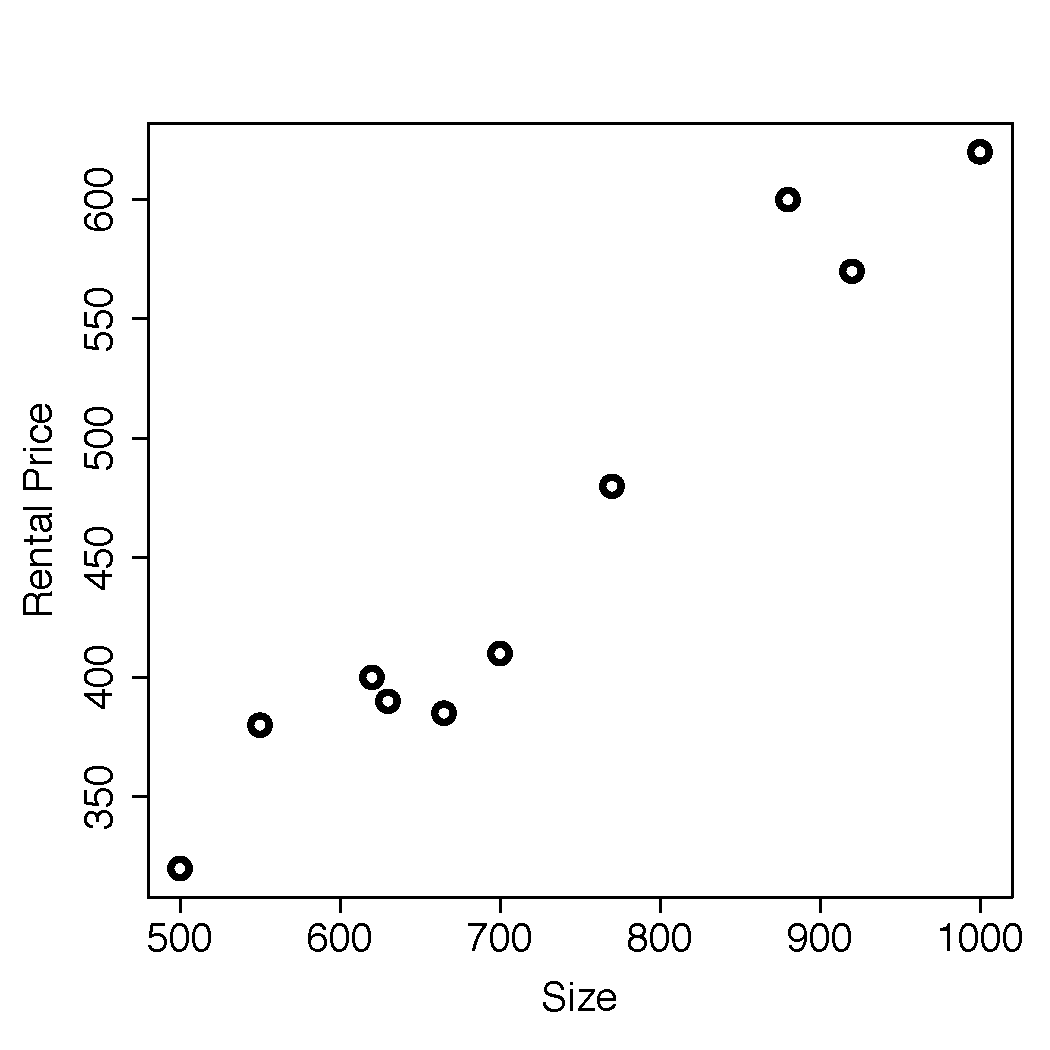
\includegraphics[width=0.75\textwidth]{./images/linearRegressionDemoDataset.pdf}
\end{center}
\caption{A scatter plot of the \featN{Size} and \featN{Rental Price} features from the office rentals dataset.}
\label{fig:officeSizesAndPrices}
\end{figure}
\end{frame} 



 \begin{frame} 
 \begin{itemize}
 	\item From the scatter plot it appears that there is a linear relationship between the \featN{Size} and \featN{Rental Price}.
	\item The equation of a line can be written as:	
		\begin{center}
		\begin{equation}
			y = mx + b 
		\end{equation}\label{eqn:line}
		\end{center}
\end{itemize}
\end{frame}

\begin{frame}
	\begin{itemize}
		\item The scatter plot below shows the same scatter plot as shown in Figure \ourRef{fig:officeSizesAndPrices} with a simple linear model added to capture the relationship between office sizes and office rental prices. 
		\item This model is:
	\end{itemize}
\begin{equation*}
\featN{Rental~Price} = 6.47 + 0.62 \times \featN{Size}
\end{equation*}
\begin{figure}[htb]
\begin{center}
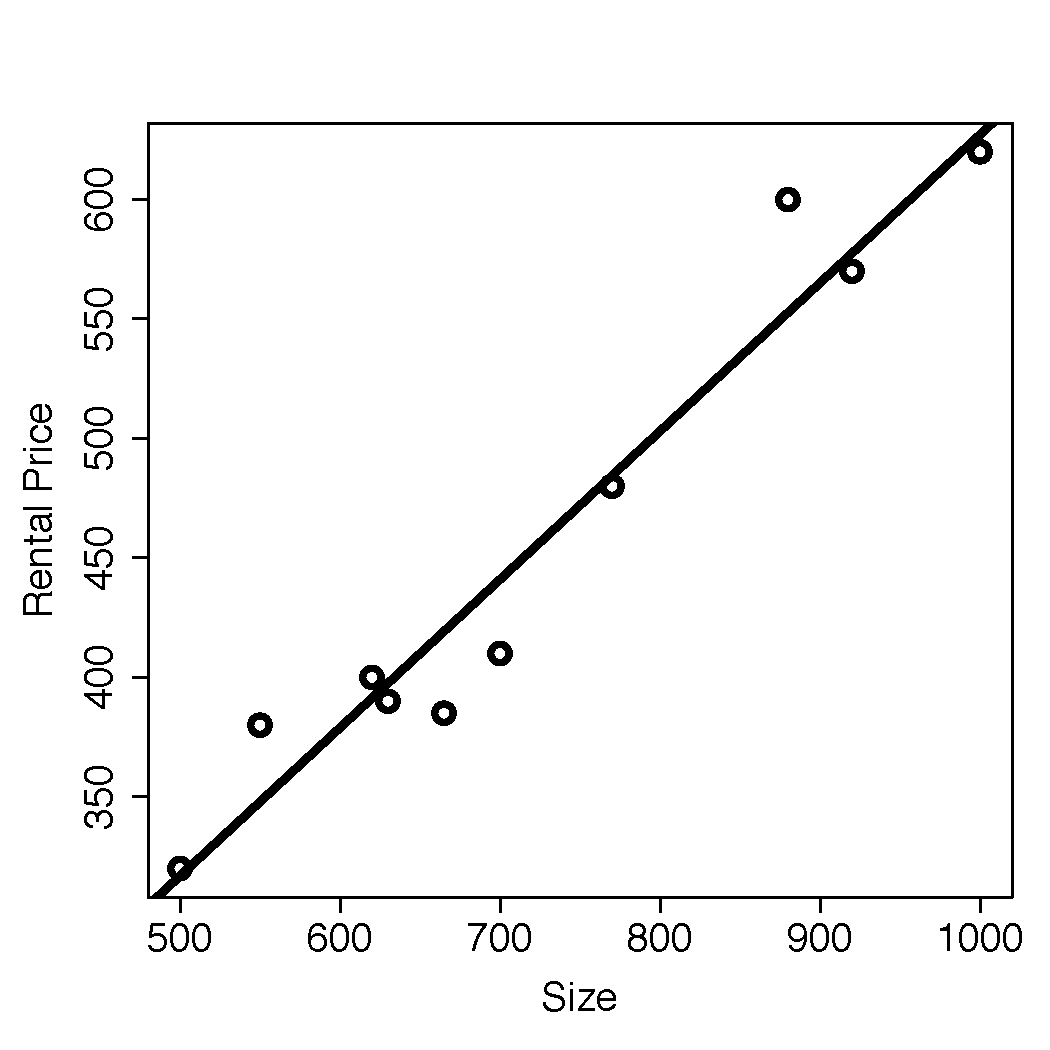
\includegraphics[width=0.4\textwidth]{./images/linearRegressionDemoFinalModel.pdf}
\label{fig:officeSizesAndPricesWithModel}
\end{center}
\end{figure}
\end{frame} 


 \begin{frame} 
\begin{equation*}
\featN{Rental~Price} = 6.47 + 0.62 \times \featN{Size}
\end{equation*}
\begin{itemize}
	\item Using this model determine the expected rental price of the $730$ square foot office:
\pause
 \begin{eqnarray*}
\featN{Rental~Price} & = & 6.47 + 0.62 \times 730 \\
& = & 459.07
\end{eqnarray*}
\end{itemize}
\end{frame} 

 \begin{frame} 
\begin{center}
\begin{equation}
\mathbb{M}_{\mathbf{w}}(d) = \mathbf{w}[0] + \mathbf{w}[1] \times \mathbf{d}[1] \label{eq:simpleLinearRegression}
\end{equation}
\end{center}
\end{frame}

\subsection{Measuring Error}

 \begin{frame} 
 \begin{figure}[htb]
\begin{center}
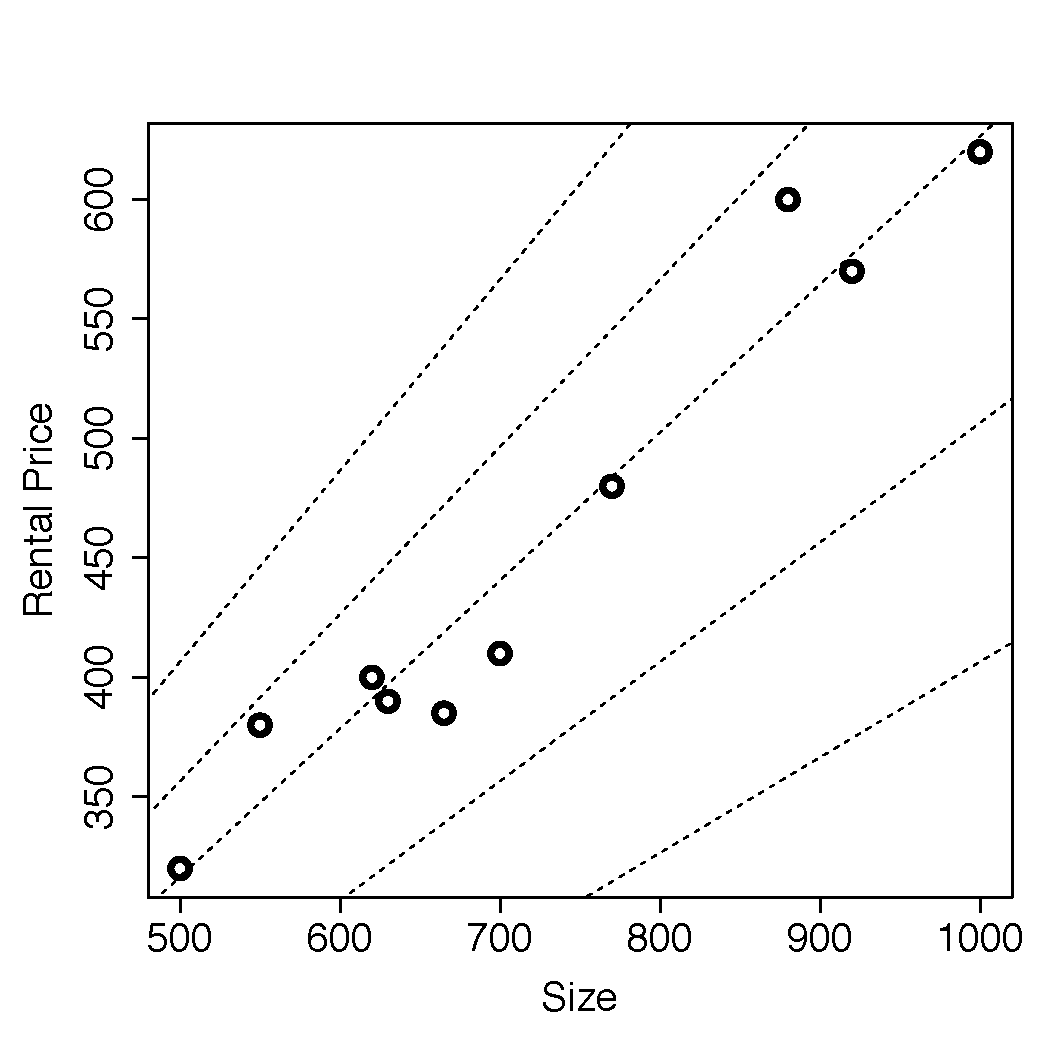
\includegraphics[width=0.5\textwidth]{./images/linearRegressionDemoMultipleModels.pdf}
\caption{A scatter plot of the \featN{Size} and \featN{Rental Price} features from the office rentals dataset. A collection of possible simple linear regression models capturing the relationship between these two features are also shown. For all models $\mathbf{w}[0]$ is set to $6.47$. From top to bottom the models use $0.4$, $0.5$, $0.62$, $0.7$ and $0.8$ respectively for $\mathbf{w}[1]$.}
\label{fig:officeSizesAndPricesWithMultipleModels}
\end{center}
\end{figure}
\end{frame} 
		
\begin{frame}
\begin{figure}[htb]
\begin{center}
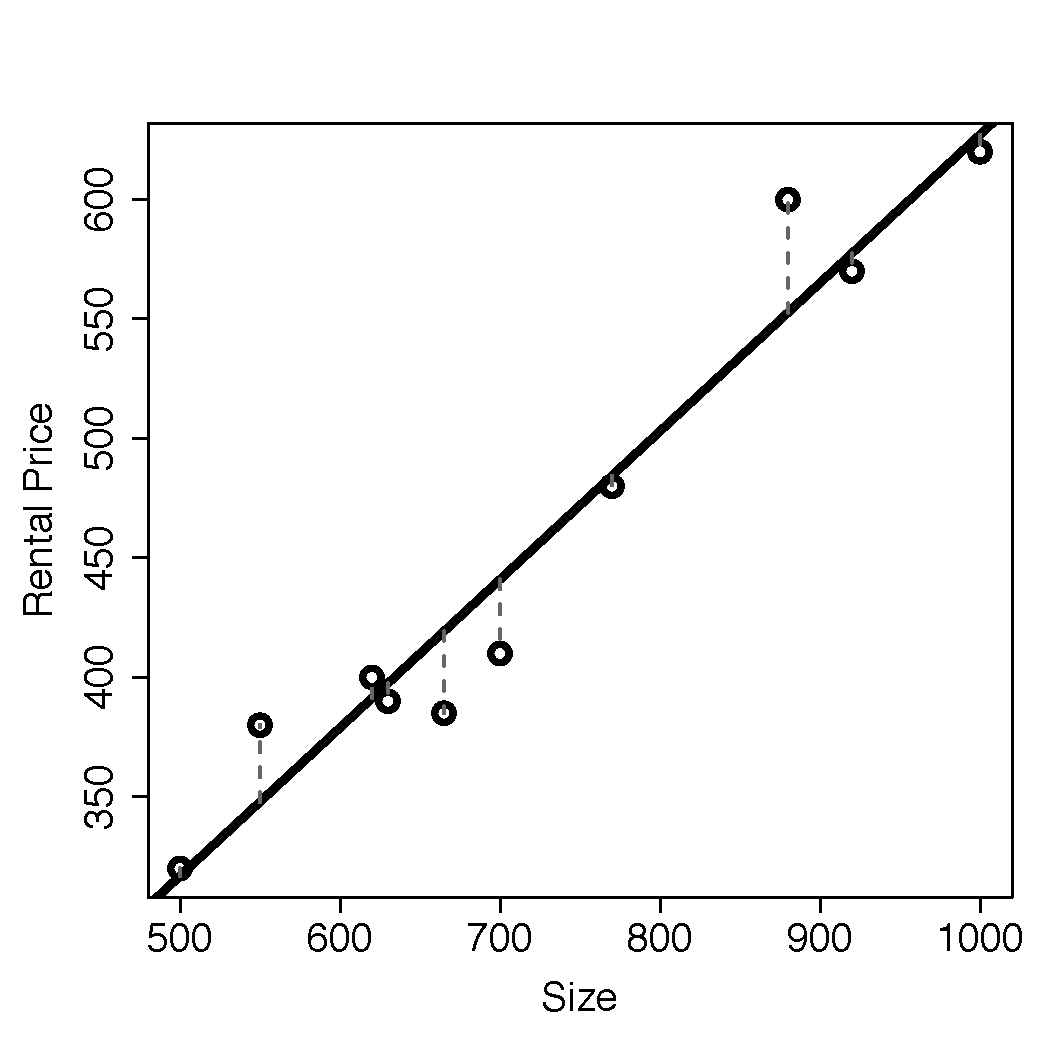
\includegraphics[width=0.6\textwidth]{./images/linearRegressionDemoFinalModelWithErrorDropdowns_mod.pdf}
\caption{A scatter plot of the \featN{Size} and \featN{Rental Price} features from the office rentals dataset showing a candidate prediction model (with $\mathbf{w}[0] = 6.47$ and $\mathbf{w}[1] = 0.62$) and the resulting errors.}
\label{fig:officeSizesAndPricesWithModelAndErrors}
\end{center}
\end{figure}
\end{frame} 

 \begin{frame} 
\begin{eqnarray}
L_2(\mathbb{M}_{\mathbf{w}}, \mathcal{D}) & = & \frac{1}{2} \sum_{i=1}^{n} \left(t_i - \mathbb{M}_{\mathbf{w}}(\mathbf{d}_i[1])\right)^2 \\
								  & = & \frac{1}{2} \sum_{i=1}^{n} \left(t_i - (\mathbf{w}[0] + \mathbf{w}[1]\times\mathbf{d}_i[1])\right)^2 
\label{eq:l2LossFunc}
\end{eqnarray}
\end{frame} 

 \begin{frame} 
\begin{table}
	\caption{Calculating the sum of squared errors for the candidate model (with $\mathbf{w}[0] = 6.47$ and $\mathbf{w}[1] = 0.62$) making predictions for the the office rentals dataset.}
	\centering
			\begin{footnotesize}
	\begin{tabular}{r r r r r }
		\hline
				\textbf{} & \textbf{\featN{Rental}} & \textbf{Model} & \textbf{Error} & \textbf{Squared} \\
		\textbf{ID} & \textbf{\featN{Price}} & \textbf{Prediction} & \textbf{Error} & \textbf{Error} \\
		\hline
		1 & 320	&	316.79	&	3.21	&	10.32	\\
		2 & 380	&	347.82	&	32.18	&	1,035.62	\\
		3 & 400	&	391.26	&	8.74	&	76.32	\\
		4 & 390	&	397.47	&	-7.47	&	55.80	\\
		5 & 385	&	419.19	&	-34.19	&	1,169.13	\\
		6 & 410	&	440.91	&	-30.91	&	955.73	\\
		7 & 480	&	484.36	&	-4.36	&	19.01	\\
		8 & 600	&	552.63	&	47.37	&	2,243.90	\\
		9 & 570	&	577.46	&	-7.46	&	55.59	\\
		10 &	620	&	627.11	&	-7.11	&	50.51	\\
		\hline
		 \multicolumn{4}{r}{\textbf{Sum}} &	\textbf{5,671.64}	\\
		 \multicolumn{4}{r}{\textbf{Sum of squared errors ($\mathbf{Sum}/2$)}} &	\textbf{2,835.82}	\\
		\hline
	\end{tabular}
			\end{footnotesize}
\label{tab:officeSizesAndPricesSumOfSquaredErrorsExample}
\end{table}
\end{frame} 


\subsection{Error Surfaces}

\begin{frame}
	\begin{itemize}
		\item For every possible combination of weights, $\mathbf{w}[0]$ and $\mathbf{w}[1]$, there is a corresponding sum of squared errors value that can be joined together to make a surface. 
	\end{itemize}

\begin{figure}[htb]
\begin{center}
	\subfigure[]{\label{fig:officeSizesAndPricesErrorSurface}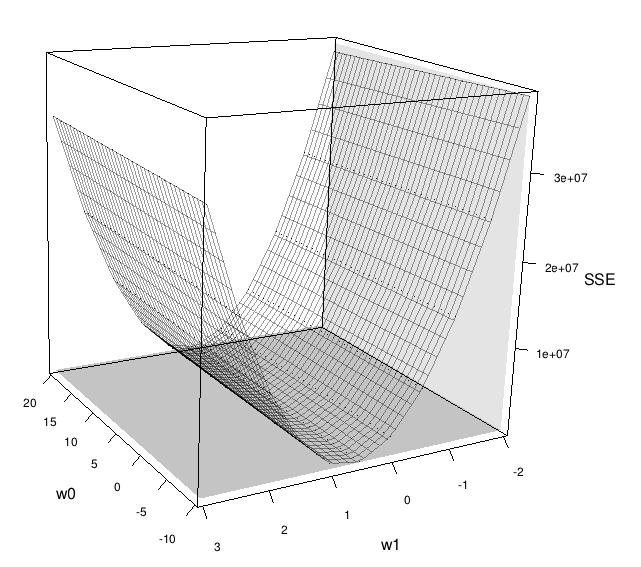
\includegraphics[width=0.35\textwidth]{./images/officePricesErrorSurface3.png}}
	\subfigure[]{\label{fig:officeSizesAndPricesErrorContour}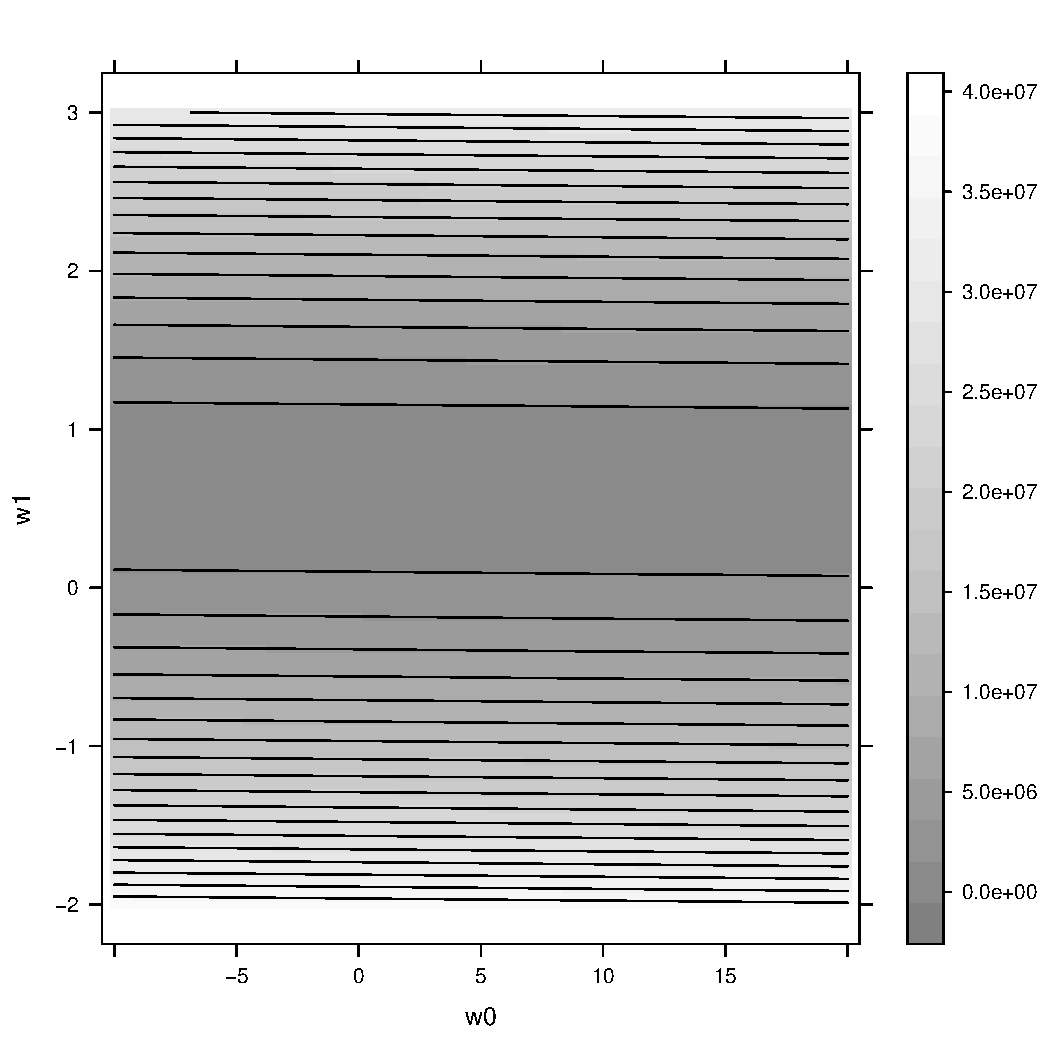
\includegraphics[width=0.25\textwidth]{./images/linearRegressionDemoLevelPlot.pdf}}
\caption{(a) A 3D surface plot and (b) a contour plot of the error surface generated by plotting the sum of squared errors value for the office rentals training set for each possible combination of values for $\mathbf{w}[0]$ (from the range $[-10, 20]$) and $\mathbf{w}[1]$ (from the range $[-2, 3]$).}
\label{fig:officeSizesAndPricesError}
\end{center}
\end{figure}
		
\end{frame}

\begin{frame}
	\begin{itemize}
		\item The $x$-$y$ plane is known as a \keyword{weight space} and the surface is known as an \keyword{error surface}. 
		\item \alert{The model that best fits the training data is the model corresponding to the lowest point on the error surface.}
	\end{itemize}
\end{frame}

\begin{frame} 
\begin{itemize}
\item Using Equation \ourEqRef{eq:l2LossFunc} we can formally define this point on the error surface as the point at which:
\begin{center}
\begin{eqnarray}
\frac{\partial}{\partial \mathbf{w}[0]} \frac{1}{2} \sum_{i=1}^{n} (t_i - (\mathbf{w}[0] + \mathbf{w}[1] \times \mathbf{d}_i[1]))^2 = 0
\label{eq:w0PartialDerivEquals0}
\end{eqnarray}
and 
\begin{eqnarray}
\frac{\partial}{\partial \mathbf{w}[1]} \frac{1}{2} \sum_{i=1}^{n} (t_i - (\mathbf{w}[0] + \mathbf{w}[1] \times \mathbf{d}_i[1]))^2 = 0
\label{eq:w1PartialDerivEquals0}
\end{eqnarray}
\end{center}
\item There are a number of different ways to find this point. 
\item We will describe a \keyword{guided search} approach known as the \keyword{gradient descent} algorithm. 
\end{itemize}
\end{frame} 


\SectionSlide{Standard Approach: Multivariate Linear Regression with Gradient Descent}

\subsection{Multivariate Linear Regression}

 \begin{frame} 
\begin{table}
	\caption{A dataset that includes office rental prices and a number of descriptive features for 10 Dublin city-center offices.}
	\centering
	\begin{footnotesize}
	\begin{tabular}{r r r r r r }
		\hline
				~	 & ~	 & ~ & \featN{Broadband} & \featN{Energy} & \featN{Rental} \\
		\featN{ID}	 & \featN{Size}	 & \featN{Floor} & \featN{Rate} & \featN{Rating} & \featN{Price} \\
		\hline
1 & 500	&	4	&	8	&	C	&	320	\\
2 & 550	&	7	&	50	&	A	&	380	\\
3 & 620	&	9	&	7	&	A	&	400	\\
4 & 630	&	5	&	24	&	B	&	390	\\
5 & 665	&	8	&	100	&	C	&	385	\\
6 & 700	&	4	&	8	&	B	&	410	\\
7 & 770	&	10	&	7	&	B	&	480	\\
8 & 880	&	12	&	50	&	A	&	600	\\
9 & 920	&	14	&	8	&	C	&	570	\\
10 & 1,000	&	9	&	24	&	B	&	620	\\
		\hline
	\end{tabular}
	\end{footnotesize}
\label{tab:officeSizesAndPrices}
\end{table}
\end{frame} 

\begin{frame}
\begin{itemize}
\item We can define a multivariate linear regression model as:
\begin{eqnarray}
\mathbb{M}_{\mathbf{w}}(\mathbf{d}) & = & \mathbf{w}[0] + \mathbf{w}[1] \times \mathbf{d}[1] + \dots + \mathbf{w}[m] \times \mathbf{d}[m] \\
& = & \mathbf{w}[0] + \sum_{j=1}^{m} \mathbf{w}[j] \times \mathbf{d}[j] 
\label{eqn:basciMultiVariateReg}
\end{eqnarray}
\end{itemize}
\end{frame} 

\begin{frame}
\begin{itemize}
\item We can make Equation \ourEqRef{eqn:basciMultiVariateReg} look a little neater by inventing a dummy descriptive feature, $\mathbf{d}[0]$, that is always equal to $1$:
\end{itemize}
\begin{eqnarray}
\mathbb{M}_{\mathbf{w}}(\mathbf{d}) & = & \mathbf{w}[0]\times \mathbf{d}[0] + \mathbf{w}[1] \times \mathbf{d}[1] + \ldots + \mathbf{w}[m] \times \mathbf{d}[m] \\
	& = & \sum_{j=0}^{m} \mathbf{w}[j]\times \mathbf{d}[j] \label{eqn:multiVariateRegression1}\\
    & = & \mathbf{w} \cdot \mathbf{d} \label{eqn:multiVariateRegression2}
\end{eqnarray}
\end{frame} 

 \begin{frame} 
 \begin{itemize}
\item The sum of squared errors loss function, $L_2$, definition that we gave in Equation \ourEqRef{eq:l2LossFunc} changes only very slightly to reflect the new regression equation:
\begin{eqnarray}
L_2(\mathbb{M}_{\mathbf{w}},\mathcal{D}) & = & \frac{1}{2}\sum_{i=1}^{n} (t_i - \mathbb{M}_{\mathbf{w}}(\mathbf{d}_i))^2 \\
								  & = &  \frac{1}{2} \sum_{i=1}^{n} (t_i - (\mathbf{w} \cdot \mathbf{d}_i))^2 
\label{eq:l2LossFuncMultiVariate}
\end{eqnarray}
\end{itemize}
\end{frame} 

 \begin{frame} 
 \begin{itemize}
\item This multivariate model allows us to include all but one of the descriptive features in Table \ourRef{tab:officeSizesAndPricesSumOfSquaredErrorsExample} in a regression model to predict office rental prices. 
\item The resulting multivariate regression model equation is:
\end{itemize}
\begin{eqnarray*}
	\featN{Rental Price} = \mathbf{w}[0] & + &  \mathbf{w}[1] \times \featN{Size} + \mathbf{w}[2] \times \featN{Floor} \\
	 & + &  \mathbf{w}[3] \times \featN{Broadband~Rate}
\end{eqnarray*}
\end{frame} 


 \begin{frame} 
\begin{itemize}
\item We will see in the next section how the best-fit set of weights for this equation are found, but for now we will set:
\begin{itemize}
\item $\mathbf{w}[0] = -0.1513$, 
\item $\mathbf{w}[1] = 0.6270$, 
\item $\mathbf{w}[2] = -0.1781$,
\item $\mathbf{w}[3] = 0.0714$. 
\end{itemize}
 \item This means that the model is rewritten as:
\end{itemize}
\begin{eqnarray*}
	\featN{Rental Price} =  -0.1513 	 &+&  0.6270 \times \featN{Size}\\
			& - &  0.1781 \times \featN{Floor} \\	 														& + & 0.0714 \times \featN{Broadband~Rate}
\end{eqnarray*}
\end{frame} 

 \begin{frame} 
\begin{itemize}
\item Using this model:
\end{itemize}
 \begin{eqnarray*}
	\featN{Rental Price} =  -0.1513 	 &+&  0.6270 \times \featN{Size}\\
			& - &  0.1781 \times \featN{Floor} \\	 														& + & 0.0714 \times \featN{Broadband~Rate}
\end{eqnarray*}
\begin{itemize}
\item we can, for example, predict the expected rental price of a $690$ square foot office on the $11^{th}$ floor of a building with a broadband rate of $50$ Mb per second as:
\end{itemize}
\begin{eqnarray*}
	\featN{Rental~Price} & = & \alert{?}\\
\end{eqnarray*}
\end{frame} 

 \begin{frame} 
\begin{itemize}
\item Using this model:
\end{itemize}
 \begin{eqnarray*}
	\featN{Rental Price} =  -0.1513 	 &+&  0.6270 \times \featN{Size}\\
			& - &  0.1781 \times \featN{Floor} \\	 														& + & 0.0714 \times \featN{Broadband~Rate}
\end{eqnarray*}
\begin{itemize}
\item we can, for example, predict the expected rental price of a $690$ square foot office on the $11^{th}$ floor of a building with a broadband rate of $50$ Mb per second as:
\end{itemize}
\begin{eqnarray*}
	\featN{Rental~Price} & = & -0.1513 + 0.6270 \times 690\\
	& ~& ~-0.1781 \times 11 + 0.0714 \times 50 \\
	 & = & 434.0896
\end{eqnarray*}
\end{frame} 

\subsection{Gradient Descent}

 \begin{frame} 
\begin{figure}[htb]
\begin{center}
	\subfigure[]{\label{fig:gradientDescentErrorExamplesSurface}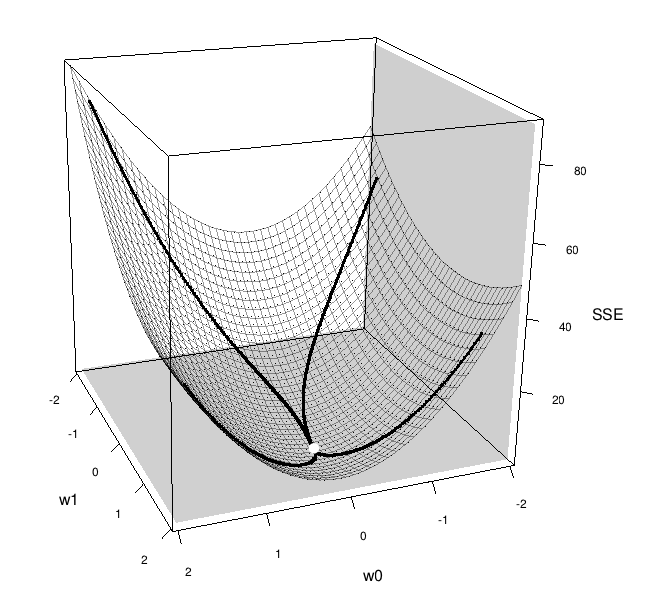
\includegraphics[width=0.45\textwidth]{./images/linearRegressionDemoErrorSurfaceMultipleStartsO.png}}
	\subfigure[]{\label{fig:gradientDescentErrorExamplesContour}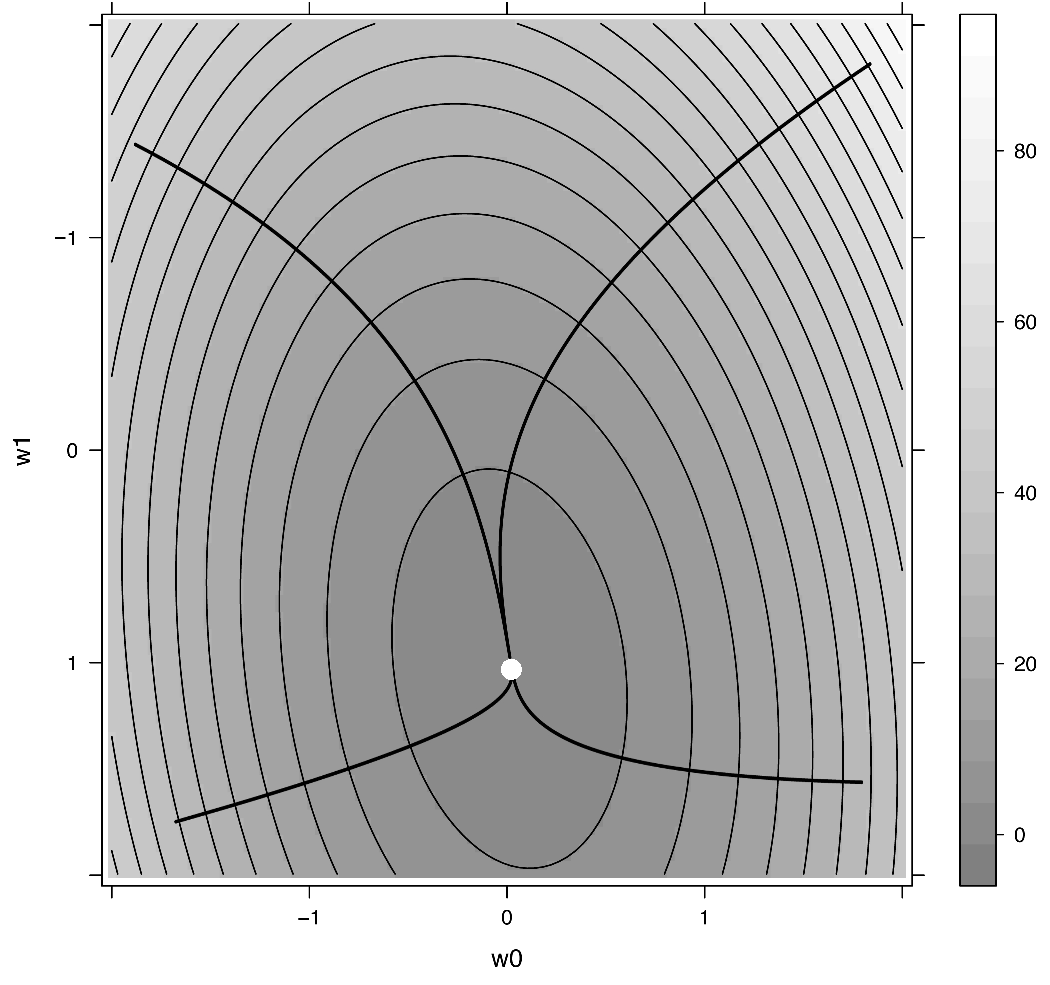
\includegraphics[width=0.45\textwidth]{./images/linearRegressionDemoLevelPlotMultipleStartsO.pdf}}
\caption{(a) A 3D surface plot and (b) a contour plot of the same error surface. The lines indicate the path that the gradient decent algorithm would take across this error surface from different starting positions to the global minimum - marked as the white dot in the centre.}
\label{fig:gradientDescentErrorExamples}
\end{center}
\end{figure}
\end{frame} 

	
\begin{frame}[plain]
\begin{itemize}
\item The journey across the error surface that is taken by the gradient descent algorithm when training the simple version of the office rentals example - involving just \featN{Size} and \featN{Rental Price}.
\end{itemize}

\begin{figure}[htb]
\begin{center}
	\subfigure[]{\label{fig:officeRentalsErrorSurfaceJourneySurface}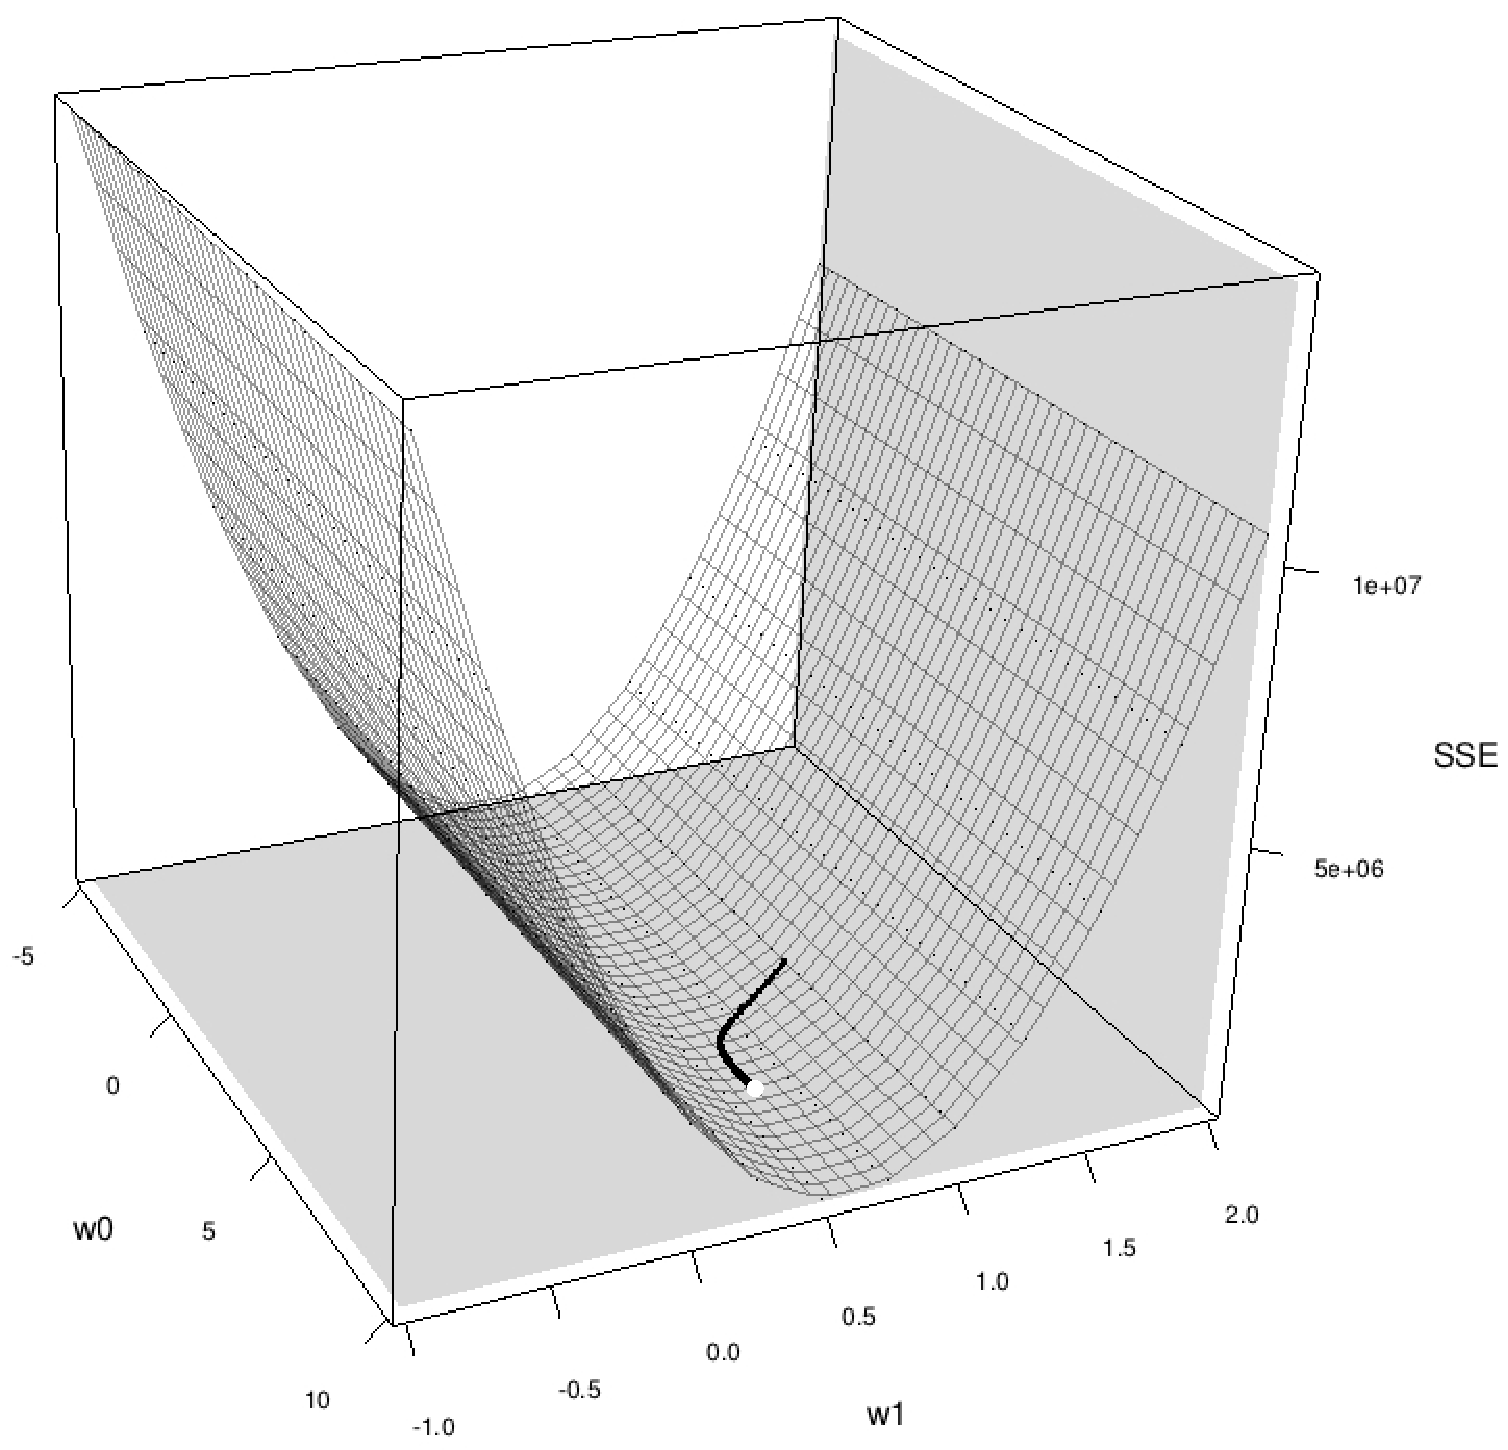
\includegraphics[width=0.45\textwidth]{./images/officeRentalsErrorSurfaceJourneyO.pdf}}
	\subfigure[]{\label{fig:officeRentalsErrorSurfaceJourneyContour}\includegraphics[width=0.45\textwidth]{./images/officeRentalsLevelPlotO_mod.pdf}}
\caption{(a) A 3D surface plot and (b) a contour plot of the error surface for the office rentals dataset showing the path that the gradient descent algorithm takes towards the best fit model.}
\label{fig:officeRentalsErrorSurfaceJourney}
\end{center}
\end{figure}
\end{frame}

 \begin{frame} [plain]
\begin{figure}[htb]
\begin{center}
	\subfigure{\label{fig:officeGradientDescentSmallMultiples0}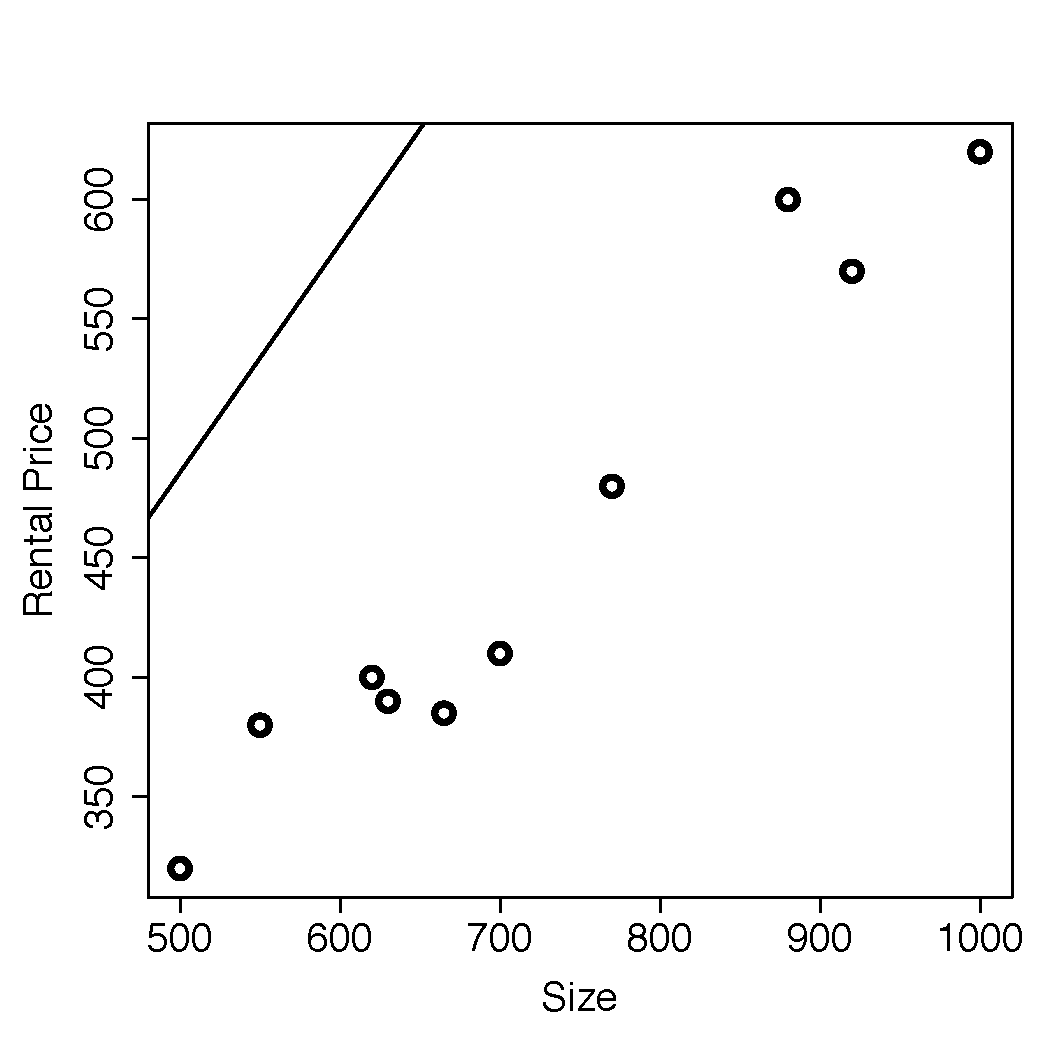
\includegraphics[width=0.27\textwidth]{./images/linearRegressionDemo0.pdf}}
	\subfigure{\label{fig:officeGradientDescentSmallMultiples1}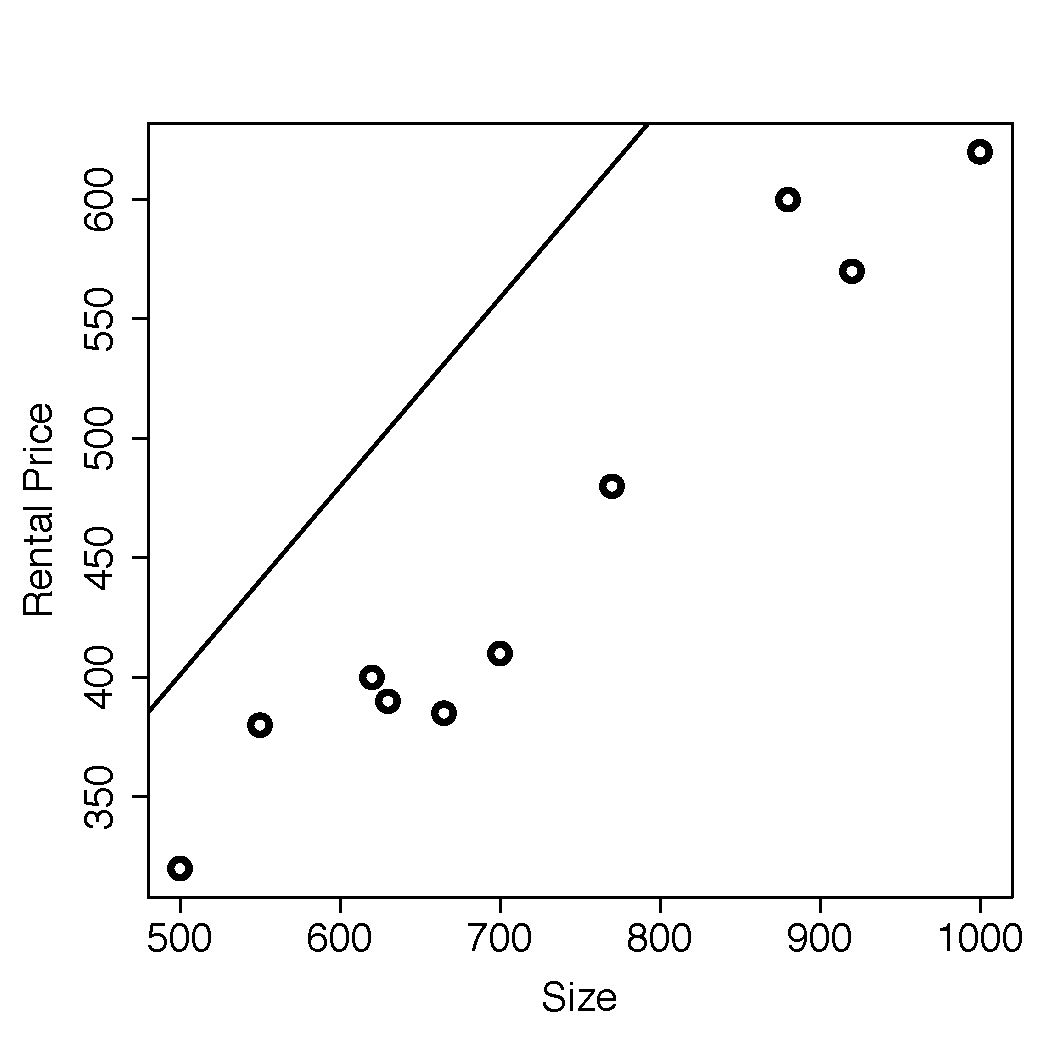
\includegraphics[width=0.27\textwidth]{./images/linearRegressionDemo6.pdf}}
	\subfigure{\label{fig:officeGradientDescentSmallMultiples2}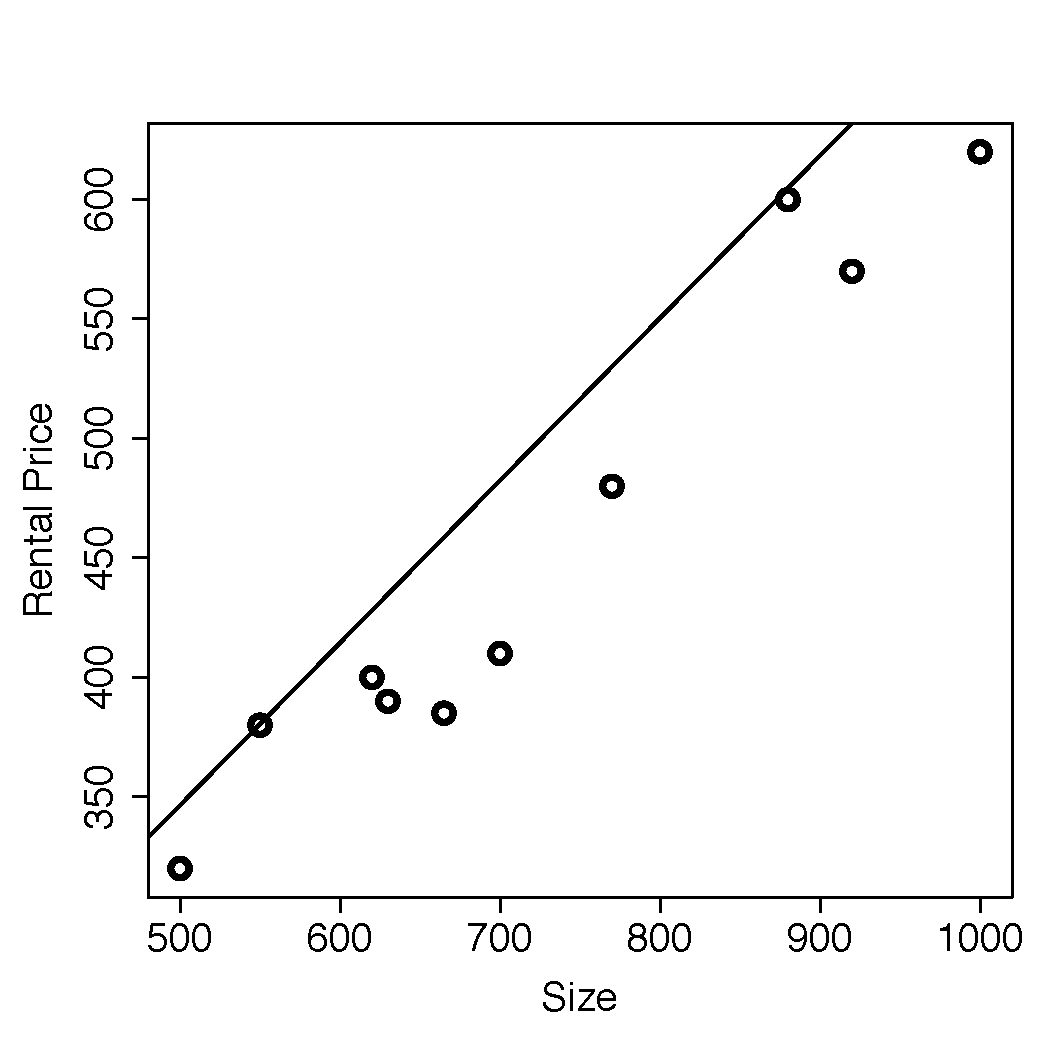
\includegraphics[width=0.27\textwidth]{./images/linearRegressionDemo15.pdf}}
	\subfigure{\label{fig:officeGradientDescentSmallMultiples3}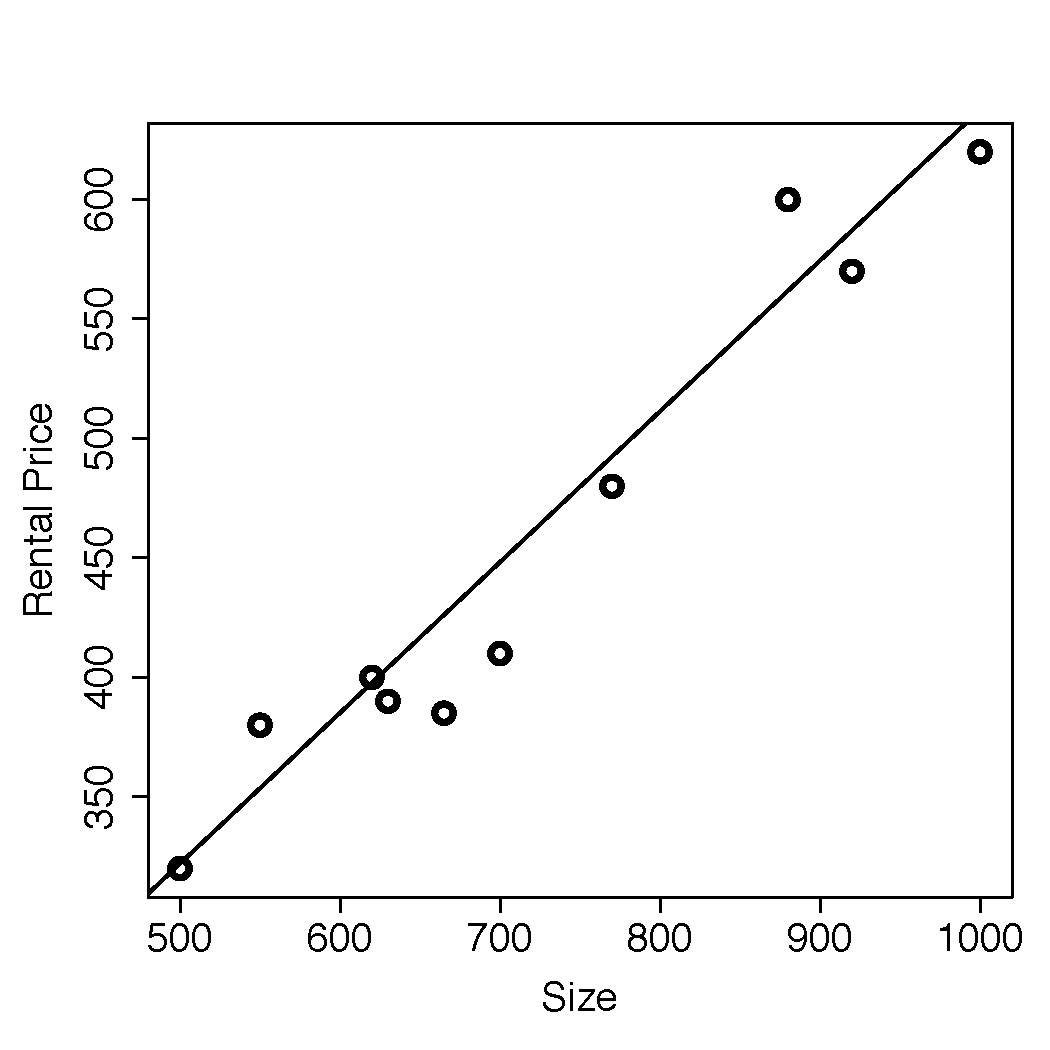
\includegraphics[width=0.27\textwidth]{./images/linearRegressionDemo30.pdf}}
	\subfigure{\label{fig:officeGradientDescentSmallMultiples4}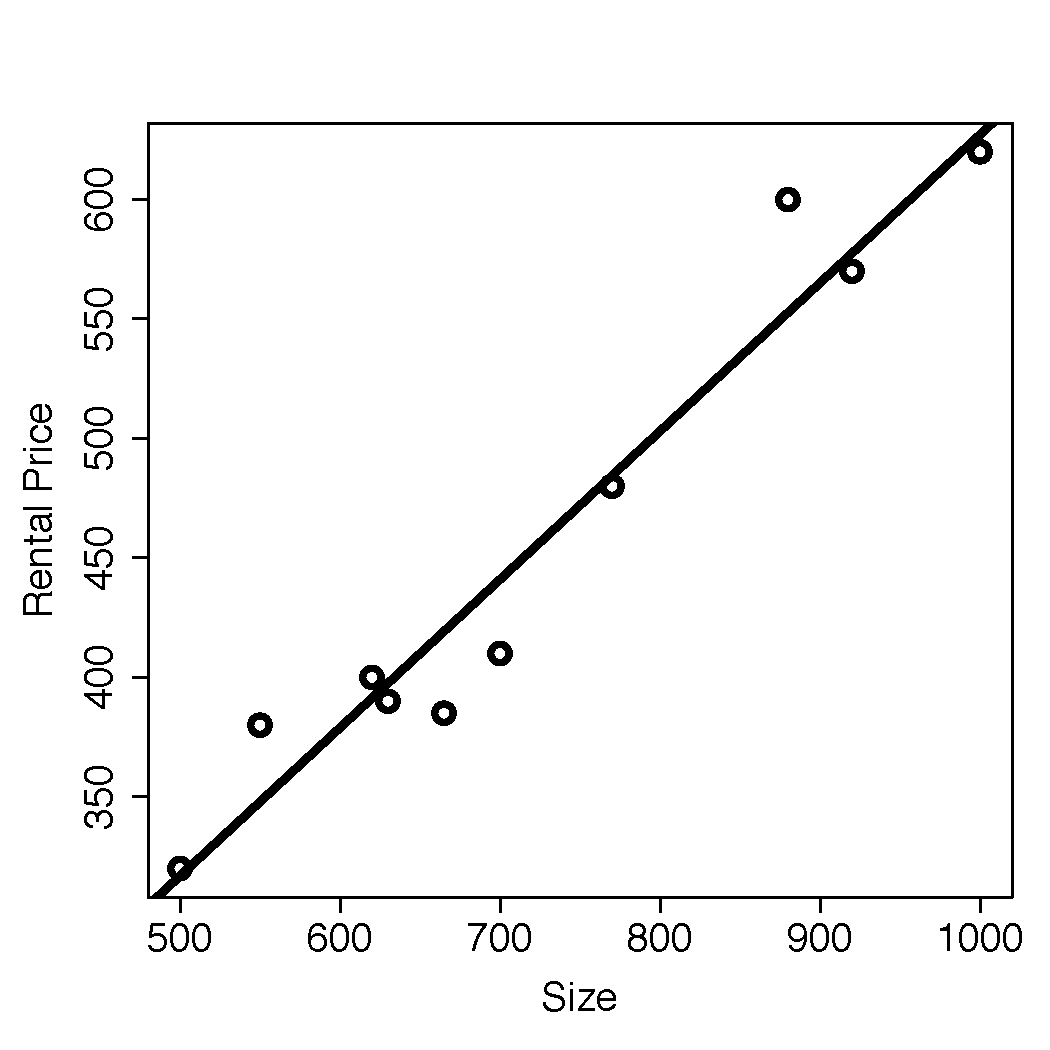
\includegraphics[width=0.27\textwidth]{./images/linearRegressionDemoFinalModel.pdf}}
	\subfigure{\label{fig:officeGradientDescentSmallMultiples5}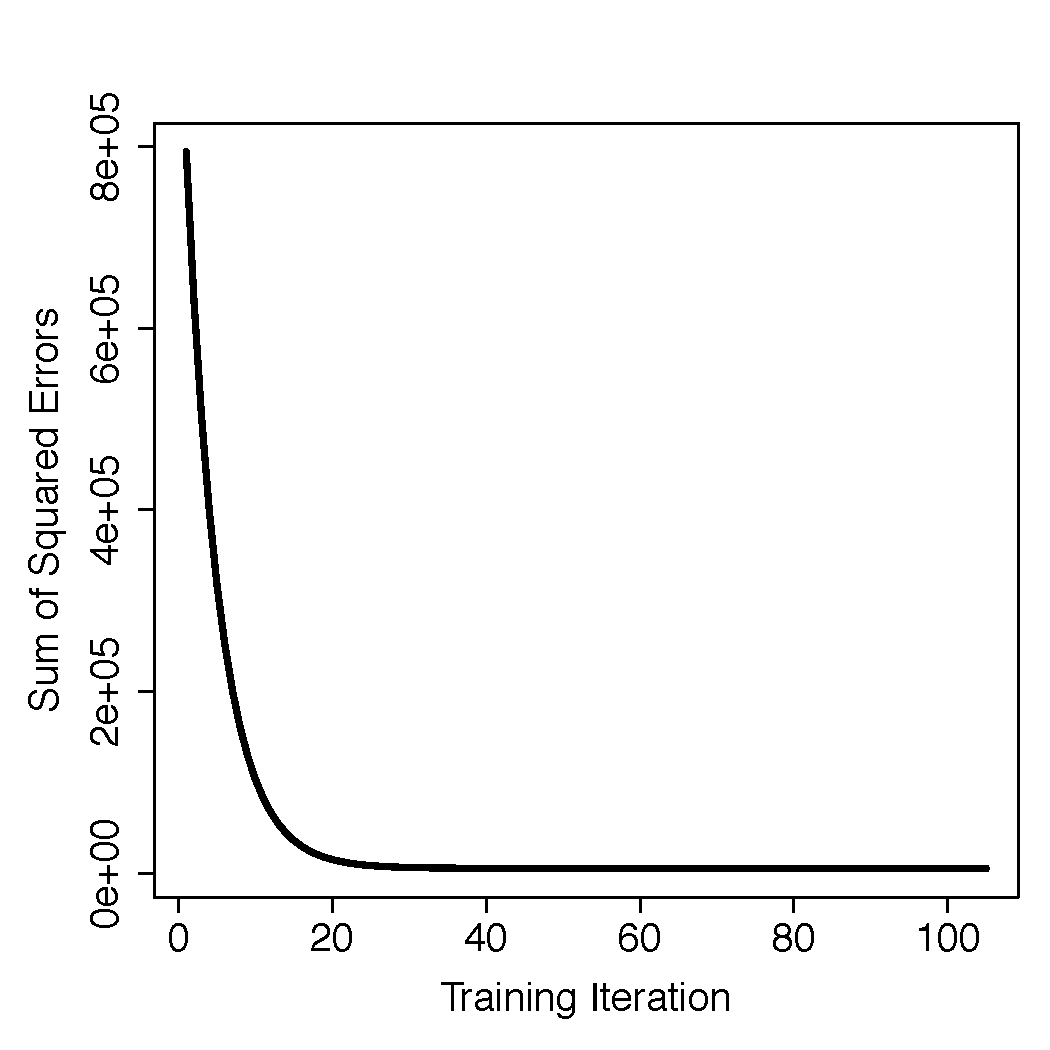
\includegraphics[width=0.27\textwidth]{./images/linearRegressionDemoErrorJourney.pdf}}		
\caption{A selection of the simple linear regression models developed during the gradient descent process for the office rentals dataset. The final panel shows the sum of squared error values generated during the gradient descent process. }
\label{fig:officeGradientDescentSmallMultiples}
\end{center}
\end{figure}
\end{frame} 




\begin{frame}
\begin{algorithmic}[1]
\REQUIRE set of training instances $\mathcal{D}$
\REQUIRE a learning rate $\alpha$ that controls how quickly the algorithm converges
\REQUIRE a function, \textbf{errorDelta}, that determines the direction in which to adjust a given weight, $\mathbf{w}[j]$, so as to move down the slope of an error surface determined by the dataset, $\mathcal{D}$ 
\REQUIRE a convergence criterion that indicates that the algorithm has completed 
\STATE $\mathbf{w} \leftarrow $ random starting point in the weight space
\REPEAT
	\FOR{each $\mathbf{w}[j]$ in $\mathbf{w}$}
		\STATE $\mathbf{w}[j] \leftarrow \mathbf{w}[j] + \alpha \times \textbf{errorDelta}(\mathcal{D}, \mathbf{w}[j])$ \label{algLine:weightUpdateRule}
	\ENDFOR	
\UNTIL{convergence occurs} 
\end{algorithmic}
\begin{itemize}
\item \alert{The gradient descent algorithm for training multivariate linear regression models.}
\end{itemize}
\end{frame}

\begin{frame}
\begin{itemize}
\item The most important part to the gradient descent algorithm is Line Rule 4 on which the weights are updated. 
\begin{equation*}
\mathbf{w}[j] \leftarrow \mathbf{w}[j] + \alpha \times \textbf{errorDelta}(\mathcal{D}, \mathbf{w}[j])
\end{equation*}
\item Each weight is considered independently and for each one a small adjustment is made by adding a small \indexkeyword{delta} value to the current weight, $\mathbf{w}[j]$. 
\item This adjustment should ensure that the change in the weight leads to a move \textit{downwards} on the error surface. 
\end{itemize}
\end{frame}
 
\begin{frame}
\begin{itemize} 
 \item Imagine for a moment that our training dataset, $\mathcal{D}$ contains \alert{just one training} example: $(\mathbf{d}, t)$
 \item The gradient of the error surface is given as the partial derivative of $L_2$ with respect to each weight, $\mathbf{w}[j]$:

 \end{itemize}
  
\begin{eqnarray}
\frac{\partial}{\partial \mathbf{w}[j]} L_2 \left( \mathbb{M}_{\mathbf{w}}, \mathcal{D} \right) & =  & \frac{\partial}{\partial \mathbf{w}[j]} \left( \frac{1}{2} \left(t - \mathbb{M}_{\mathbf{w}} \left( \mathbf{d} \right) \right) ^2 \right) \label{eqn:gradDesc1} \\
						& = & (t - \mathbb{M}_{\mathbf{w}}(\mathbf{d})) \times \frac{\partial}{\partial \mathbf{w}[j]} (t - \mathbb{M}_{\mathbf{w}}(\mathbf{d})) \label{eqn:gradDesc2} \\
						& = & (t - \mathbb{M}_{\mathbf{w}}(\mathbf{d})) \times \frac{\partial}{\partial \mathbf{w}[j]} (t - (\mathbf{w} \cdot \mathbf{d})) \label{eqn:gradDesc3} \\
						& = & (t - \mathbb{M}_{\mathbf{w}}(\mathbf{d})) \times \alert{-\mathbf{d}[j]} \label{eqn:gradDesc4} 
\end{eqnarray}

\end{frame} 

 \begin{frame} 
 \begin{itemize}
	\item Adjusting the calculation to take into account multiple training instances:
\end{itemize}
\begin{equation*}
	\frac{\partial}{\partial \mathbf{w}[j]} L_2(\mathbb{M}_{\mathbf{w}}, \mathcal{D})  =   \sum_{i=1}^{n} \left(\left(t_i - \mathbb{M}_{\mathbf{w}}\left(\mathbf{d}_i\right)\right)\times \mathbf{d}_i[j]\right)
\end{equation*}
\begin{itemize}
	\item We use this equation to define the \textbf{errorDelta} in our gradient descent algorithm.
\end{itemize}
\begin{equation*}
	\mathbf{w}[j] \leftarrow \mathbf{w}[j] + \alpha \underbrace{\sum_{i=1}^{n} \left(\left(t_i - \mathbb{M}_{\mathbf{w}}\left(\mathbf{d}_i\right)\right)\times d_i[j]\right)}_{\alert{errorDelta(\mathcal{D}, \mathbf{w}[j])}}
\end{equation*}
\end{frame} 

\subsection{Choosing Learning Rates \& Initial Weights}

\begin{frame}
\begin{itemize}
\item The learning rate, \alert{$\alpha$}, determines the size of the adjustment made to each weight at each step in the process. 
\item Unfortunately, choosing learning rates is not a well defined science. 
\item Most practitioners use rules of thumb and trial and error. 
\end{itemize}
\end{frame}

 \begin{frame} 
\begin{figure}[!htb]
\begin{center}
	\subfigure[]{\label{fig:learningRateSmall}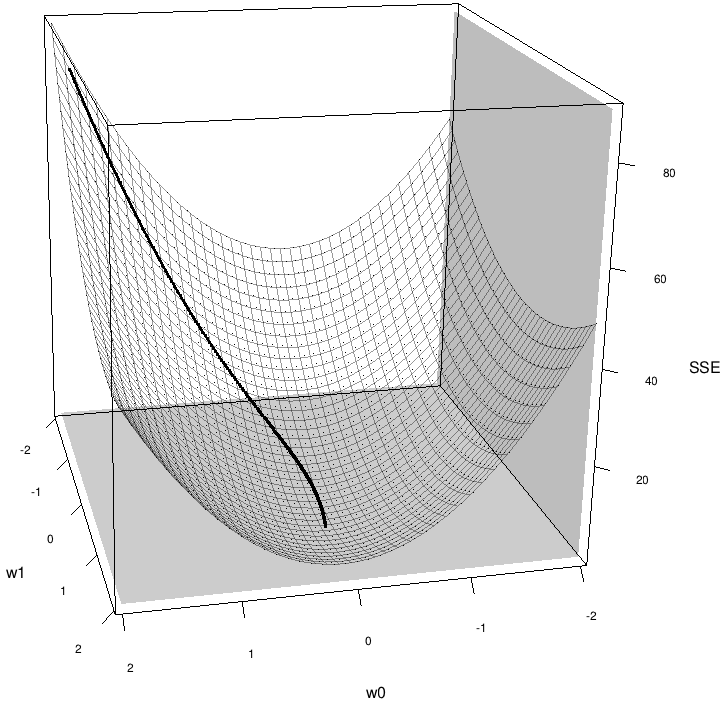
\includegraphics[width=0.32\textwidth]{./images/linearRegressionDemoErrorSurfaceJourneyDifferentLearningRates0_002.png}}
	\subfigure[]{\label{fig:learningRateMedium}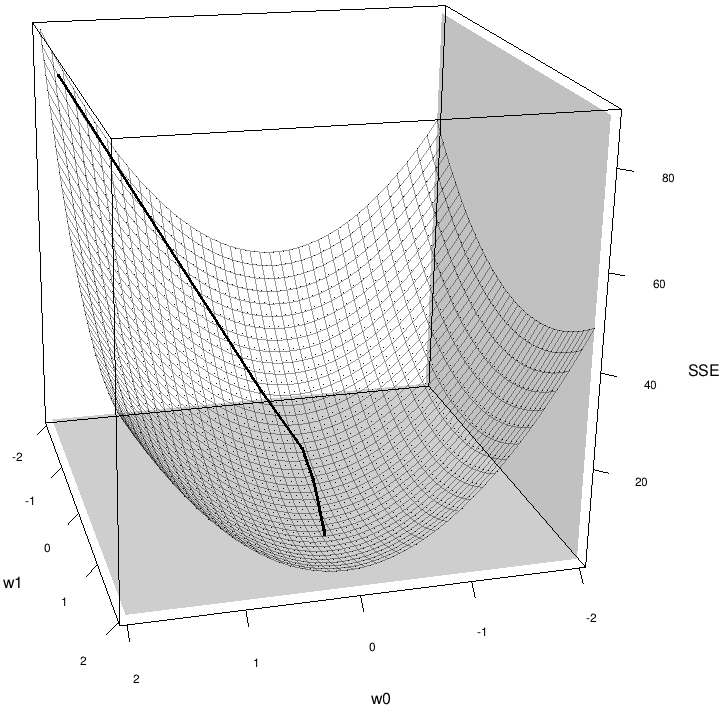
\includegraphics[width=0.32\textwidth]{./images/linearRegressionDemoErrorSurfaceJourneyDifferentLearningRates0_08.png}}
	\subfigure[]{\label{fig:learningRateLarge}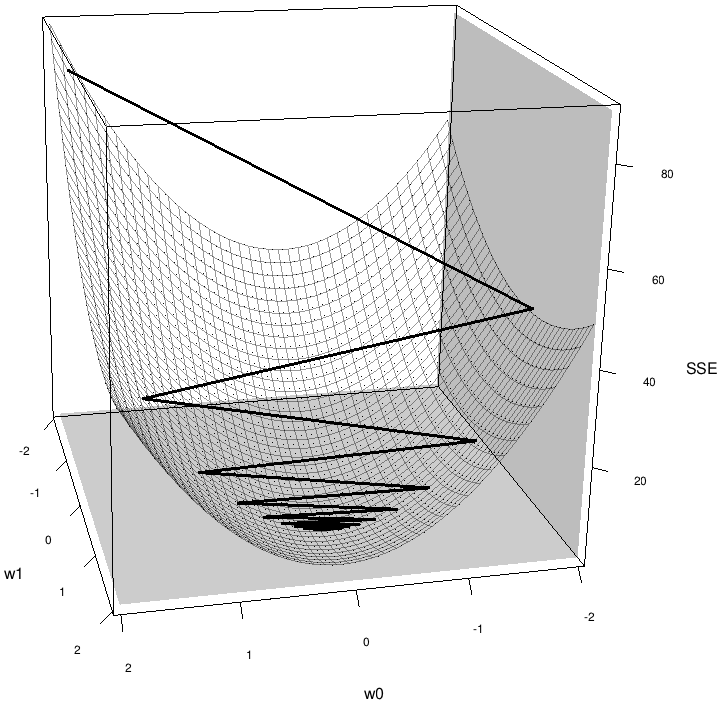
\includegraphics[width=0.32\textwidth]{./images/linearRegressionDemoErrorSurfaceJourneyDifferentLearningRates0_18.png}}	
%	\subfigure[]{\label{fig:learningRateSmallErrorGraph}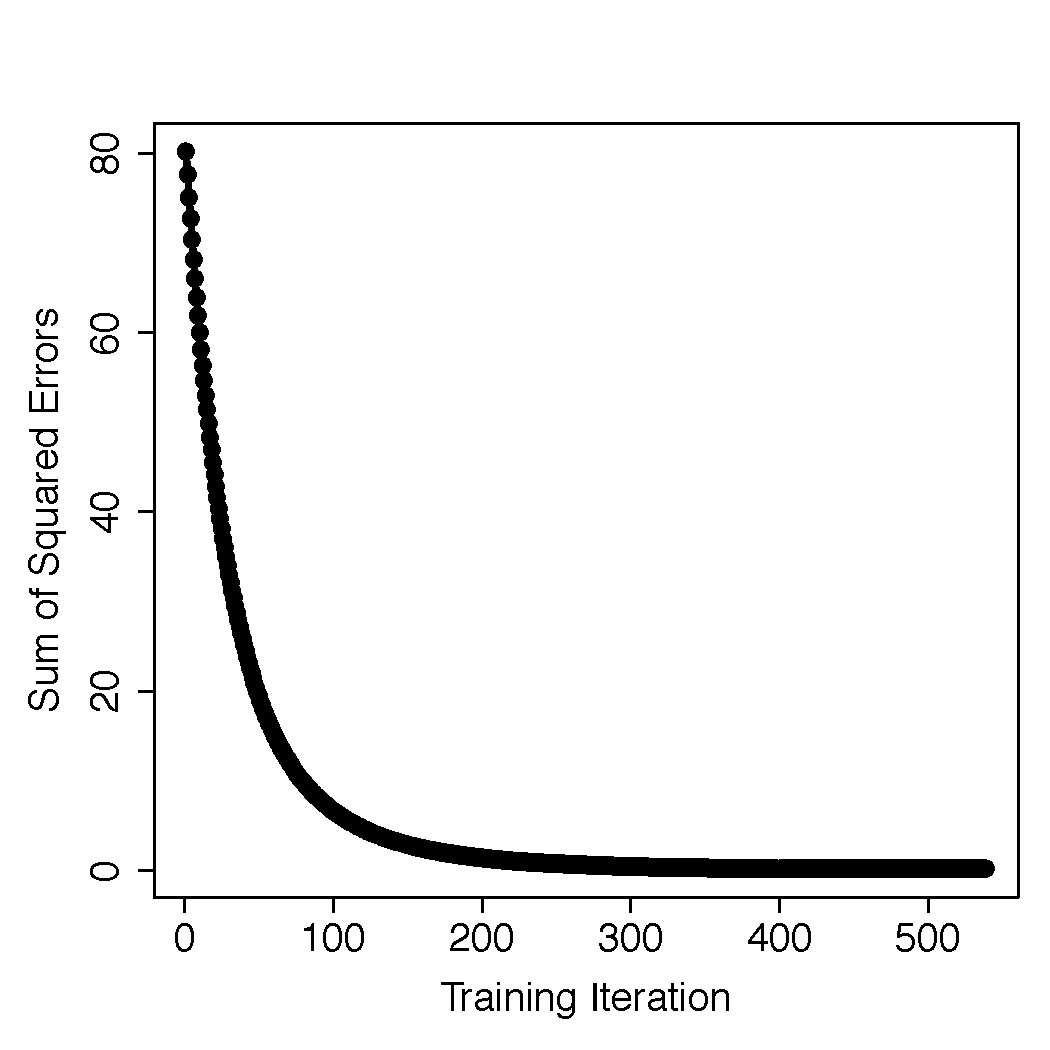
\includegraphics[width=0.25\textwidth]{./images/linearRegressionDemoErrorJourneyDifferentLearningRates0_002.pdf}}
%	\subfigure[]{\label{fig:learningRateMediumErrorGraph}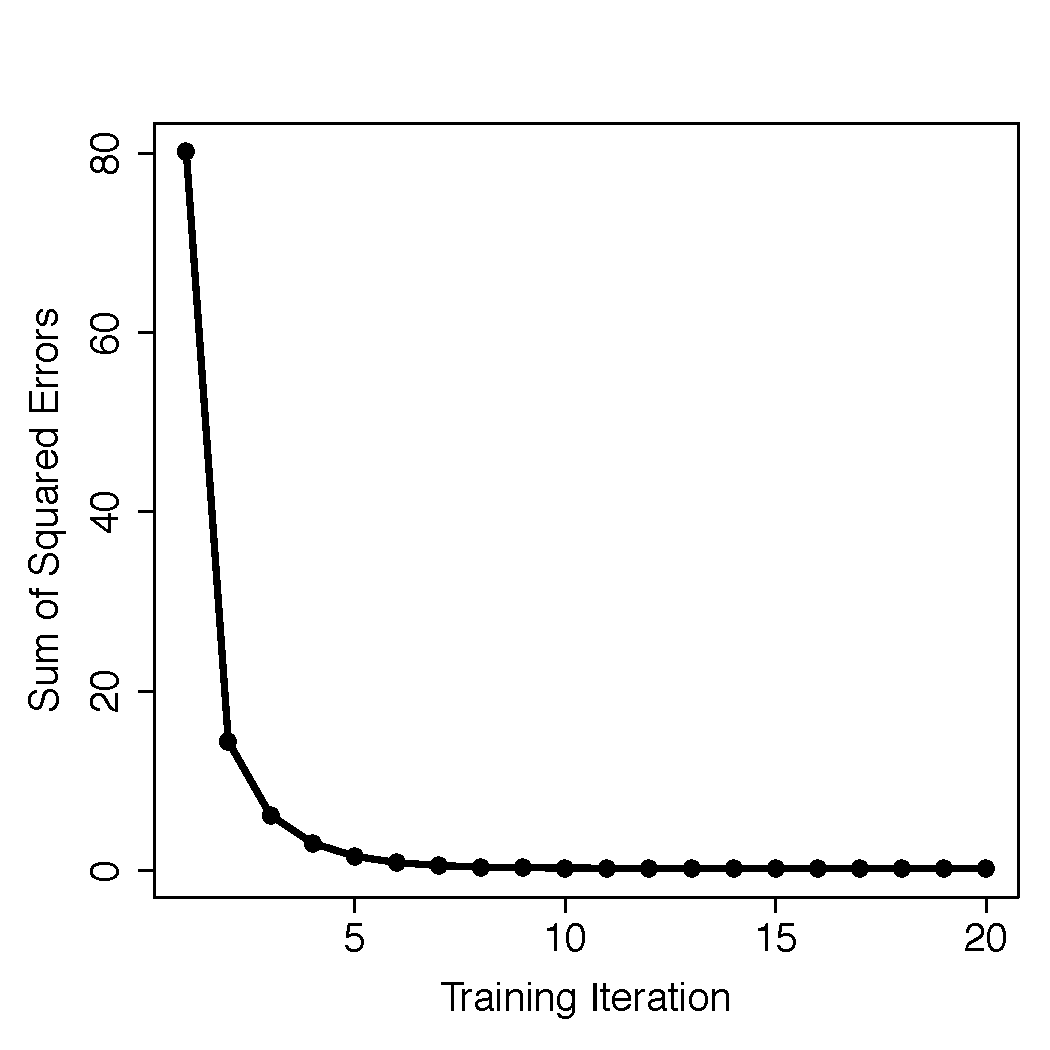
\includegraphics[width=0.25\textwidth]{./images/linearRegressionDemoErrorJourneyDifferentLearningRates0_08.pdf}}
%	\subfigure[]{\label{fig:learningRateLargeErrorGraph}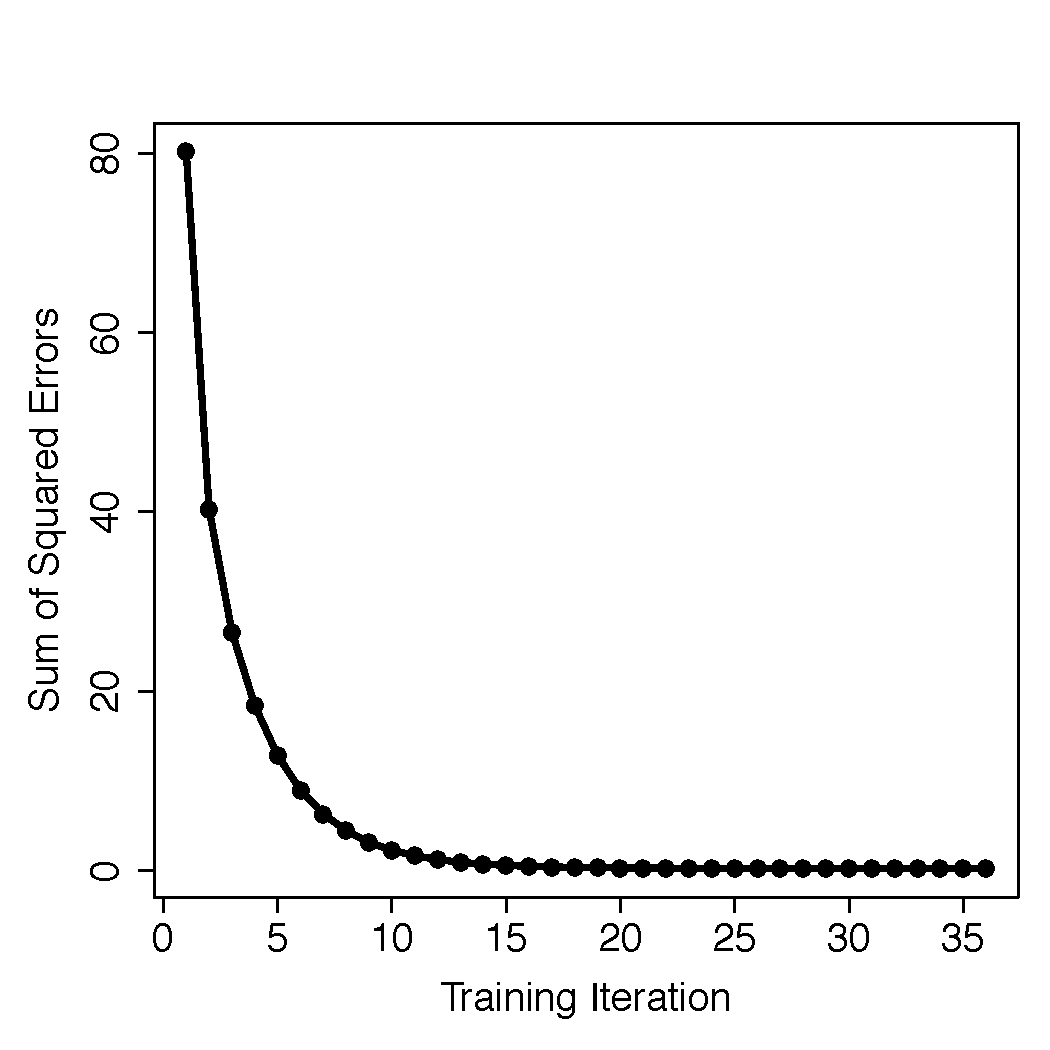
\includegraphics[width=0.25\textwidth]{./images/linearRegressionDemoErrorJourneyDifferentLearningRates0_18.pdf}}	
\caption{Plots of the journeys made across the error surface for the simple office rentals prediction problem for different learning rates: (a) a very small learning rate ($0.002$), (b) a medium learning rate ($0.08$) and (c) a very large learning rate ($0.18$). }
\label{fig:learningRates}
\end{center}
\end{figure}
\end{frame} 

\begin{frame}
\begin{itemize}
\item A typical range for learning rates is $[0.00001, 10]$ 
\item Based on empirical evidence, choosing random initial weights uniformly from the range $[-0.2, 0.2]$ tends to work well.
\end{itemize}
\end{frame}

\subsection{A Worked Example}

 \begin{frame} 
 \begin{itemize}
 	\item We are now in a position to build a linear regression model that uses all of the continuous descriptive features in the office rentals dataset. 
	\item The general structure of the model is:
\end{itemize}
\begin{eqnarray*}
	\featN{Rental~Price}  =  \mathbf{w}[0] 	& + &  \mathbf{w}[1] \times \featN{Size} + \mathbf{w}[2] \times \featN{Floor}	\\
 														& + &  \mathbf{w}[3] \times \featN{Broadband~Rate}
\end{eqnarray*}
\end{frame} 

 \begin{frame} 
\begin{table}
	\caption{The \textbf{office rentals dataset}: a dataset that includes office rental prices and a number of descriptive features for 10 Dublin city-centre offices.}
	\centering
	\begin{footnotesize}
	\begin{tabular}{r r r r r r }
		\hline
				\textbf{}	 & \textbf{}	 & \textbf{} & \textbf{\featN{Broadband}} & \textbf{\featN{Energy}} & \textbf{\featN{Rental}} \\
		\textbf{\featN{ID}}	 & \textbf{\featN{Size}}	 & \textbf{\featN{Floor}} & \textbf{\featN{Rate}} & \textbf{\featN{Rating}} & \textbf{\featN{Price}} \\
		\hline
1 & 500	&	4	&	8	&	C	&	320	\\
2 & 550	&	7	&	50	&	A	&	380	\\
3 & 620	&	9	&	7	&	A	&	400	\\
4 & 630	&	5	&	24	&	B	&	390	\\
5 & 665	&	8	&	100	&	C	&	385	\\
6 & 700	&	4	&	8	&	B	&	410	\\
7 & 770	&	10	&	7	&	B	&	480	\\
8 & 880	&	12	&	50	&	A	&	600	\\
9 & 920	&	14	&	8	&	C	&	570	\\
10 & 1,000	&	9	&	24	&	B	&	620	\\
		\hline
	\end{tabular}
	\end{footnotesize}
\label{tab:officeSizesAndPrices}
\end{table}
\end{frame} 

\begin{frame}
\begin{itemize}
\item For this example let's assume that:
	\begin{itemize}
		\item $\alpha = 0.00000002$ 
	\end{itemize}
	\begin{footnotesize}
		\begin{tabular}{c c c c c c c c}
			\multicolumn{8}{c}{\textbf{Initial Weights}} \\
			\hline
			$\mathbf{w}[0]$: &	-0.146	& 	$\mathbf{w}[1]$:	&	0.185	 & $\mathbf{w}[2]$: &	-0.044	 & $\mathbf{w}[3]$: &	0.119 \\
			\hline
	\end{tabular}
	\end{footnotesize}
\end{itemize}
\end{frame}

\begin{frame}
\begin{footnotesize}
\resizebox{\linewidth}{!}{
	\begin{tabular}{ c c c c c | c c c c }
		\multicolumn{9}{ c }{\textbf{Iteration 1}}	\\
		\hline
%				\textbf{} & \textbf{\featN{Rental}} & \textbf{} & \textbf{} & \textbf{Squared} & \textbf{$\textbf{errorDelta}$} & \textbf{$\textbf{errorDelta}$} & \textbf{$\textbf{errorDelta}$} & \textbf{$\textbf{errorDelta}$} \\
				~ & \featN{Rental} & ~ & ~ & Squared & \multicolumn{4}{c}{$\mathbf{errorDelta(\mathcal{D}, w[i])}$} \\
%		\textbf{ID} & \textbf{\featN{Price}} & \textbf{Pred.} & \textbf{Error} & \textbf{Error} & \textbf{$(\mathcal{D}, \mathbf{w}[0])$} & \textbf{$(\mathcal{D}, \mathbf{w}[1])$} & \textbf{$(\mathcal{D}, \mathbf{w}[2])$} & \textbf{$(\mathcal{D}, \mathbf{w}[3])$} \\
		\featN{ID} & \featN{Price} & Pred. & Error & Error & $\mathbf{w}[0]$ & $\mathbf{w}[1]$ & $\mathbf{w}[2]$ & $\mathbf{w}[3]$ \\
		\hline
	
1	&	320	&	93.26	&	226.74	&	51411.08	&	226.74	&	113370.05	&	906.96	&	1813.92	\\
2	&	380	&	107.41	&	272.59	&	74307.70	&	272.59	&	149926.92	&	1908.16	&	13629.72	\\
3	&	400	&	115.15	&	284.85	&	81138.96	&	284.85	&	176606.39	&	2563.64	&	1993.94	\\
4	&	390	&	119.21	&	270.79	&	73327.67	&	270.79	&	170598.22	&	1353.95	&	6498.98	\\
5	&	385	&	134.64	&	250.36	&	62682.22	&	250.36	&	166492.17	&	2002.91	&	25036.42	\\
6	&	410	&	130.31	&	279.69	&	78226.32	&	279.69	&	195782.78	&	1118.76	&	2237.52	\\
7	&	480	&	142.89	&	337.11	&	113639.88	&	337.11	&	259570.96	&	3371.05	&	2359.74	\\
8	&	600	&	168.32	&	431.68	&	186348.45	&	431.68	&	379879.24	&	5180.17	&	21584.05	\\
9	&	570	&	170.63	&	399.37	&	159499.37	&	399.37	&	367423.83	&	5591.23	&	3194.99	\\
10	&	620	&	187.58	&	432.42	&	186989.95	&	432.42	&	432423.35	&	3891.81	&	10378.16	\\
		\hline 															
			 \multicolumn{4}{r}{\textbf{Sum}} & 1067571.59	&	3185.61	&	2412073.90	&	27888.65	&	88727.43	\\
			 \multicolumn{4}{r}{\textbf{Sum of squared errors (Sum/2)}} &	533785.80	&		&		&		&		\\
%			 \multicolumn{4}{r}{(Sum/2)} &	&		&		&		&		\\

		\hline
		\end{tabular}
		}%end resize box
	\end{footnotesize}
\end{frame}


\begin{frame}
\begin{equation*}
	\mathbf{w}[j] \leftarrow \mathbf{w}[j] + \alpha \underbrace{\sum_{i=1}^{n} \left(\left(t_i - \mathbb{M}_{\mathbf{w}}\left(\mathbf{d}_i\right)\right)\times d_i[j]\right)}_{errorDelta(\mathcal{D}, \mathbf{w}[j])}
\end{equation*}
\resizebox{\textwidth}{!}{\begin{tabular}{c c c c c c c c}
			\multicolumn{8}{c}{\textbf{Initial Weights}} \\
			\hline
			$\mathbf{w}[0]$: &	-0.146	& 	$\mathbf{w}[1]$:	&	0.185	 & $\mathbf{w}[2]$: &	-0.044	 & $\mathbf{w}[3]$: &	0.119 \\
			\hline
	\end{tabular}}
\begin{example}
\begin{equation*}
	\mathbf{w}[1] \leftarrow 0.185 + 0.00000002 \times 2,412,074 = 0.23324148
\end{equation*}
\end{example}
\resizebox{\textwidth}{!}{\begin{tabular}{c c c c c c c c}
			\multicolumn{8}{c}{\textbf{New Weights (Iteration 1)}} \\
			\hline
			$\mathbf{w}[0]$: &	-0.146	& 	$\mathbf{w}[1]$:	&	0.233	 & $\mathbf{w}[2]$: &	-0.043	 & $\mathbf{w}[3]$: &	0.121 \\
			\hline
	\end{tabular}}
\end{frame}

\begin{frame}
	\begin{footnotesize}	
	\resizebox{\linewidth}{!}{
	\begin{tabular}{ c c c c c | c c c c }
		\multicolumn{9}{ c }{\textbf{Iteration 2}}	\\
		\hline
%				\textbf{} & \textbf{\featN{Rental}} & \textbf{} & \textbf{} & \textbf{Squared} & \textbf{$\textbf{errorDelta}$} & \textbf{$\textbf{errorDelta}$} & \textbf{$\textbf{errorDelta}$} & \textbf{$\textbf{errorDelta}$} \\
				~ & \featN{Rental} & ~ & ~ & Squared & \multicolumn{4}{c}{$\mathbf{errorDelta(\mathcal{D}, w[i])}$} \\
%		\textbf{ID} & \textbf{\featN{Price}} & \textbf{Pred.} & \textbf{Error} & \textbf{Error} & \textbf{$(\mathcal{D}, \mathbf{w}[0])$} & \textbf{$(\mathcal{D}, \mathbf{w}[1])$} & \textbf{$(\mathcal{D}, \mathbf{w}[2])$} & \textbf{$(\mathcal{D}, \mathbf{w}[3])$} \\
		\featN{ID} & \featN{Price} & Pred. & Error & Error & $\mathbf{w}[0]$ & $\mathbf{w}[1]$ & $\mathbf{w}[2]$ & $\mathbf{w}[3]$ \\
		\hline
	
1	&	320	&	117.40	&	202.60	&	41047.92	&	202.60	&	101301.44	&	810.41	&	1620.82	\\
2	&	380	&	134.03	&	245.97	&	60500.69	&	245.97	&	135282.89	&	1721.78	&	12298.44	\\
3	&	400	&	145.08	&	254.92	&	64985.12	&	254.92	&	158051.51	&	2294.30	&	1784.45	\\
4	&	390	&	149.65	&	240.35	&	57769.68	&	240.35	&	151422.55	&	1201.77	&	5768.48	\\
5	&	385	&	166.90	&	218.10	&	47568.31	&	218.10	&	145037.57	&	1744.81	&	21810.16	\\
6	&	410	&	164.10	&	245.90	&	60468.86	&	245.90	&	172132.91	&	983.62	&	1967.23	\\
7	&	480	&	180.06	&	299.94	&	89964.69	&	299.94	&	230954.68	&	2999.41	&	2099.59	\\
8	&	600	&	210.87	&	389.13	&	151424.47	&	389.13	&	342437.01	&	4669.60	&	19456.65	\\
9	&	570	&	215.03	&	354.97	&	126003.34	&	354.97	&	326571.94	&	4969.57	&	2839.76	\\
10	&	620	&	187.58	&	432.42	&	186989.95	&	432.42	&	432423.35	&	3891.81	&	10378.16	\\					
		\hline 															
			 \multicolumn{4}{ r}{\textbf{Sum}} &  886723.04	&	2884.32	&	2195615.84	&	25287.08	&	80023.74	\\
			  \multicolumn{4}{r}{\textbf{Sum of squared errors (Sum/2)}} &	443361.52	&		&		&		&		\\
%			  \multicolumn{4}{r}{(Sum/2)} &	&		&		&		&		\\
		\hline
	\end{tabular}
	}%end resizebox
	\end{footnotesize}
\end{frame}


\begin{frame}
\begin{equation*}
	\mathbf{w}[j] \leftarrow \mathbf{w}[j] + \alpha \underbrace{\sum_{i=1}^{n} \left(\left(t_i - \mathbb{M}_{\mathbf{w}}\left(\mathbf{d}_i\right)\right)\times d_i[j]\right)}_{errorDelta(\mathcal{D}, \mathbf{w}[j])}
\end{equation*}
\resizebox{\textwidth}{!}{\begin{tabular}{c c c c c c c c}
			\multicolumn{8}{c}{\textbf{Initial Weights (Iteration 2)}} \\
			\hline
			$\mathbf{w}[0]$: &	-0.146	& 	$\mathbf{w}[1]$:	&	0.233	 & $\mathbf{w}[2]$: &	-0.043	 & $\mathbf{w}[3]$: &	0.121 \\
			\hline
	\end{tabular}}
\begin{alertblock}{Exercise}
\begin{equation*}
	\mathbf{w}[1] \leftarrow ?, \mathbf{\alpha}=0.00000002
\end{equation*}
\end{alertblock}
\resizebox{\textwidth}{!}{\begin{tabular}{c c c c c c c c}
			\multicolumn{8}{c}{\textbf{New Weights (Iteration 2)}} \\
			\hline
			$\mathbf{w}[0]$: &	~?~	& 	$\mathbf{w}[1]$:	&	~?~	 & $\mathbf{w}[2]$: &	~?~	 & $\mathbf{w}[3]$: &	~?~ \\
			\hline
	\end{tabular}}
\end{frame}

\begin{frame}
\begin{equation*}
	\mathbf{w}[j] \leftarrow \mathbf{w}[j] + \alpha \underbrace{\sum_{i=1}^{n} \left(\left(t_i - \mathbb{M}_{\mathbf{w}}\left(\mathbf{d}_i\right)\right)\times d_i[j]\right)}_{errorDelta(\mathcal{D}, \mathbf{w}[j])}
\end{equation*}
\resizebox{\textwidth}{!}{\begin{tabular}{c c c c c c c c}
			\multicolumn{8}{c}{\textbf{Initial Weights (Iteration 2)}} \\
			\hline
			$\mathbf{w}[0]$: &	-0.146	& 	$\mathbf{w}[1]$:	&	0.233	 & $\mathbf{w}[2]$: &	-0.043	 & $\mathbf{w}[3]$: &	0.121 \\
			\hline
	\end{tabular}}
\begin{alertblock}{Exercise}
\begin{equation*}
	\mathbf{w}[1] \leftarrow -0.233 + 0.00000002 \times 2195616.08 = 0.27691232 
\end{equation*}
\end{alertblock}
\resizebox{\textwidth}{!}{\begin{tabular}{c c c c c c c c}
			\multicolumn{8}{c}{\textbf{New Weights (Iteration 2)}} \\
			\hline
			$\mathbf{w}[0]$: &	-0.145	& 	$\mathbf{w}[1]$:	&	0.277	 & $\mathbf{w}[2]$: &	-0.043	 & $\mathbf{w}[3]$: &	0.123 \\
			\hline
	\end{tabular}}
\end{frame}

\begin{frame}
\begin{itemize}
\item The algorithm then keeps iteratively applying the weight update rule  until it converges on a stable set of weights beyond which little improvement in model accuracy is possible. 
\item After $100$ iterations the final values for the weights are:
\begin{itemize}
\item  $\mathbf{w}[0] = -0.1513$, 
\item $\mathbf{w}[1] = 0.6270$,
\item  $\mathbf{w}[2] = -0.1781$
\item $\mathbf{w}[3] = 0.0714$ 
\end{itemize}
\item which results in a sum of squared errors value of $2,913.5$
\end{itemize}
\end{frame}

\section{Summary}

\begin{frame}
	\tableofcontents
\end{frame}

\end{document}
